\documentclass[a4paper, 10pt, american, titlepage]{article}

% useful packages
\usepackage[utf8]{inputenc}
\usepackage{minted}
\usepackage[american]{babel}
\usepackage{csquotes}
\usepackage{graphicx} % for images
\usepackage[gen]{eurosym} % for literally just the euro symbol

\usepackage{lipsum}   % lorem-ipsum placeholder text
\usepackage{bookmark} % links to other parts of the PDF
%\usepackage{minted}
% if we want to use a different style, here are some to look at
% https://www.overleaf.com/learn/latex/Biblatex_bibliography_styles
\usepackage[backend=biber,style=numeric,sorting=none]{biblatex}
\usepackage[page, titletoc, title]{appendix}
\usepackage[margin=1in]{geometry} % set 1in margins
\usepackage{hyperref}      % hyperlinks

% more breathing room
\linespread{1.5}
\setminted{fontsize=\small,baselinestretch=1}

% correct bad hyphenation here
\hyphenation{op-tical net-works semi-conduc-tor}

% stuff for LaTeX to know
\bibliography{references}
\graphicspath{ {./images/} } % put images in here
\title{Kyoto VR MQP Paper First Draft}
\author{William~Campbell, Cole~Granof, and Joseph~Petitti}
\date{\today}

% call it "Table of Contents" instead of just "Contents"
\addto{\captionsamerican}{\renewcommand*{\contentsname}{Table of Contents}}

\begin{document}

% set page numbers to Roman for the forematter (before the introduction)
\pagenumbering{roman}


\maketitle

\begin{abstract}
\begin{figure}[h]
	\centering
	
\includegraphics[width=\textwidth]{abstract.jpg}
	% Note: you don't actually need the part in square brackets for the caption,
	% but if you omit it the regular caption text will be used for the List of
	% Figures entry.
	\caption[\textit{Number 1, 1950 (Lavender Mist)}, Jackson Pollock]
	{\textit{Number 1, 1950 (Lavender Mist)}, Jackson Pollock, National
		Gallery of Art, Washington, D.C.}
	\label{fig:abstract}
\end{figure}
\end{abstract}

\section*{Acknowledgments}
\label{sec:acknowledgements}
\addcontentsline{toc}{section}{Acknowledgments}

We would like to thank Atticus Sims, CEO and founder of Kyoto VR, for sponsoring
this project and providing help and guidance throughout our time in Japan. His
knowledge of the history of Kinkaku-ji and Kyoto in general has been invaluable
to our experience.

We would also like to thank Inoue Hikaru for his help with translations and
researching AR technology. A special thank you to the IQP team working with
Kyoto VR, Lewis Cook, Nicole Escobar, Ahad Fareed, and Cameron Person, for
filming and editing the app trailer.

Finally, a thank you to our advisers: Professors Joshua Cuneo and Ralph Sutter.
Without their expert advice and feedback this project probably could not have
been completed.

\clearpage

\section*{Executive Summary}
\label{sec:executiveSummary}
\addcontentsline{toc}{section}{Executive Summary}


\clearpage

% now comes the table of contents, list of figures, and list of tables
% these should be single spaced
{
\linespread{1}

% add table of contents to itself
\tableofcontents
\addcontentsline{toc}{section}{Table of Contents}
\newpage

\listoffigures
\addcontentsline{toc}{section}{List of Figures}
\newpage

% we don't have any tables yet, but uncomment this when we do
%\addcontentsline{toc}{section}{List of Tables}
%\listoftables
%\newpage
}

% go back to 1.5 spacing and Arabic numbering for the rest of the paper
\pagenumbering{arabic}

\section{Introduction}
\label{sec:introduction}

The field of consumer-oriented Augmented Reality (AR) technology is just coming
into full swing, and it presents many unique opportunities for a myriad of
fields. This budding technological platform uses digital displays to augment
real-world information with computer-generated data. As the technology
progresses several disparate industries have found novel uses for it, some
becoming extremely profitable~\autocite{webster2018}. With smartphone
manufacturers investing billions into AR technology~\autocite{mason2016}, it
seems poised to be the next big digital interface.

Tourism and art are among the fields that could gain the most from AR
technology~\autocite{saenz2009, katz2018}. AR technology can provide accessible
information to tourists and art viewers that they would not be able to get any
other way.

Kinkaku-ji, the ``golden pavilion'' of Kyoto, is the perfect example of
this~\autocite{bornoff2000}.

\newpage

\section{Background}
\label{sec:background}

As smartphones and mobile technology become more prevalent, new forms of
human-computer interaction are becoming mainstream. Smartphones allow for an
unprecedented degree of connectivity with the digital world, but can also serve
as a tool for enhancing the physical world. In this section we explain the
origins and uses of some of this technology.

\subsection{What is Augmented Reality?}
\label{sec:whatIsAugmentedReality}

Augmented Reality, or AR, is a type of human-computer interface where
perceptions of the real world are enhanced by computer-generated information.
This differs from Virtual Reality (VR) in that a VR experience consists
exclusively of virtual information. In AR, virtual information is mixed with
sensory input from the real world~\autocite{carmigniani2011}. This can enhance
the user's perception of reality by providing information that would be
difficult or impossible to display through traditional means.

For example, AR can be used to display information about historical events,
places, and objects overlaid onto images of the real
world~\autocite{saenz2009}.  This provides the user with useful information
without needing to alter the real historic site.

\subsection{Current Augmented Reality Technology}
\label{sec:currentAugmentedRealityTechnology}

While preparing for this project our team researched the current state of
augmented reality technology. Smartphones are the most commonly used AR
hardware by far [citation needed]. Typically smartphone AR applications make
use of the phone's camera, accelerometer, gyroscope, and GPS sensors to
reproduce a view of the real world with virtual information layered on top of
it~\autocite{bonsor2018}.

\subsection{Augmented Reality Use Cases}
\label{sec:augmentedRealityUseCases}

Even though it is still a developing technology, augmented reality has been used
in many disparate disciplines, including data
visualization~\autocite{resnick2017}, commerce~\autocite{matney2018},
marketing~\autocite{sharma2015}, education~\autocite{stewart-smith2012}, visual
art~\autocite{katz2018}, and even archaeology~\autocite{eve2012}.

The video game industry has readily embraced augmented reality, leading to the
development of many AR games for smartphones and dedicated head-mounted
displays. Perhaps the most popular AR game, \textit{Pokémon Go}, has been
downloaded over a billion times~\autocite{webster2018}. This game makes use of
GPS and camera data to overlay game objects (in this case fictional monsters) on
top of images of the real world~\autocite{concepcion2016} (see Figure
\ref{fig:pokemonGo}).

\begin{figure}[h]
	\centering
	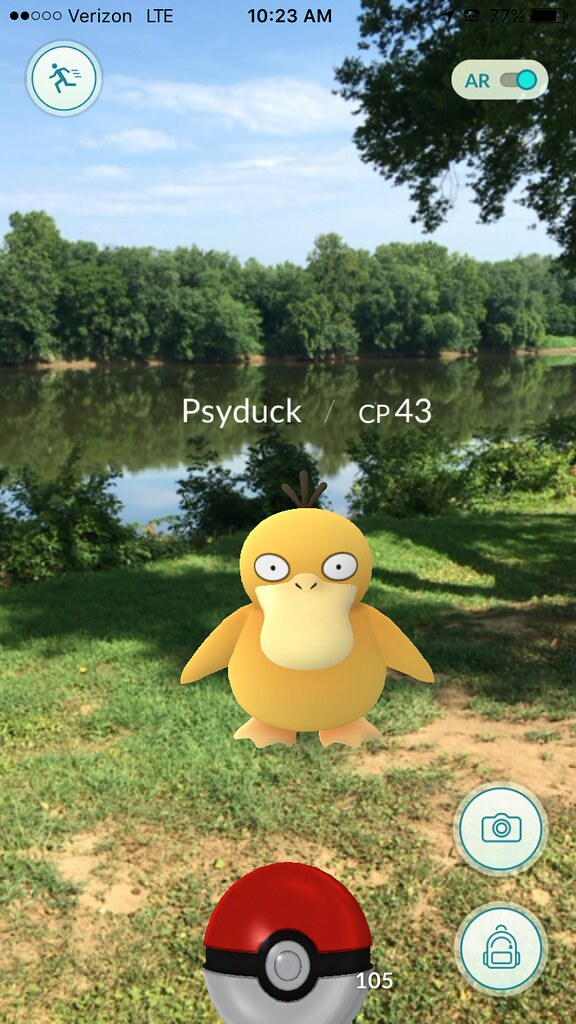
\includegraphics[width=.5\textwidth]{pokemon-go.jpg}
	\caption[A screenshot from the AR game \textit{Pokémon Go}]{A screenshot
		from the AR game \textit{Pokémon Go}~\autocite{vastateparks2016}.}
	\label{fig:pokemonGo}
\end{figure}

\subsection{Challenges of Augmented Reality}
\label{sec:challengesOfAugmentedReality}

As previously discussed, AR is a new and growing field full of opportunities.
But of course, as with anything new, our understanding of AR and how to develop
for it is limited.  And with those limitations come challenges. All sorts of
different challenges and limitations face the development and production of AR
apps. Here are some that we considered when working on our app.

Many of the applications and use cases that exist for AR right now are, simply
put, not very good. This means a few different things. For starters, many AR
apps and features available on smartphones offer very little in the way of
functionality or practicality; quite simply, they are primarily used for minor
spectacles and simple tricks~\autocite{theappsolutions2018}. For example, one
of the most popular apps to use AR, Pokemon GO, primarily uses it's AR feature
to place a Pokemon in the world aroudn you through your phone camera for you to
capture. But when it is in the world, it does not interact with anything around
it. It just floats a fixed distance away from you, simply placed on top of your
camera's video feed. 

Additionally, in many cases where AR is used, the task could be accomplished as
well or better without AR~\autocite{theappsolutions2018}. Returning to the
Pokemon GO example, when the AR feature is left on while capturing a Pokemon,
the extra power needed for this feature drains the device faster, makes it
harder to hit the Pokemon with a Pokeball due to the model drifting in the
environment, and can even slow app performance, all of which detract from the
ability to play and enjoy the game. 

One of the major problems facing AR development as a whole, and one that we ran
into as well, is limited hardware. For starters, smartphone cameras present a
major limitation. Many smartphone cameras only capture images in 2D, which can
make generating AR content in a 3D world difficult without the use of QR or
barcode markers~\autocite{geospatialworld2018}. Additionally, GPS sensors on
smartphones can also be too imprecise for good AR
tracking~\autocite{geospatialworld2018}.

The biggest hardware limitation comes from which platform to use. AR apps are
most commonly designed for smartphones due to their relatively low cost and how
accessible they are. But, as we just discussed, smartphones come with a host of
hardware limitations that make achieving satisfying AR capabilities difficult.
Additionally, AR apps for smartphones tend not to be very user-friendly, and
oftentimes even complicate the task or activity they were meant to
enhance~\autocite{theappsolutions2018}.  The alternative then is to turn to
dedicated hardware, like Microsoft's HoloLens.  But dedicated hardware like the
HoloLens is very inaccessible and expensive; Microsoft only offers developer
editions of the HoloLens, and for the incredibly steep price of
\$3,500~\autocite{microsoft2019}. 

The challenges we faced during development mirrored these that plague the
industry as a whole very accurately. We struggled with how exactly we would us
AR for our app in a way that benefit the experience as a whole, but believe the
way we've implemented it will enhance the user's experience. Hardware issues
were definitely our biggest challenge.  Only one of our phones is new enough to
run AR technology at a decent level, making testing of our application
difficult.  

\subsection{Apps for Art and Culture}
\label{sec:appsForArtAndCulture}

To explore existing AR apps for art and culture our group researched and tested
several games, experiences, and platforms related to our project.

\subsubsection{izi.TRAVEL}
\label{sec:iziTravel}

Before our project started, Kyoto VR was already using an app with a limited
form of AR for tours. The app, called izi.TRAVEL, allows users to create audio
tours with audio and image files tied to specific locations in the real
world~\autocite{izitravel2015} (see Figure \ref{fig:iziTravel}). The app is
aimed at museums and city tours~\autocite{izitravel} but can be used for tours
of historic sites too.  Kyoto VR used the platform to make an audio tour of
Kinkaku-ji, one of the most popular tourist destinations in
Japan~\autocite{bornoff2000} and an important historic heritage
site~\autocite{unesco}.

\begin{figure}[h]
	\centering
	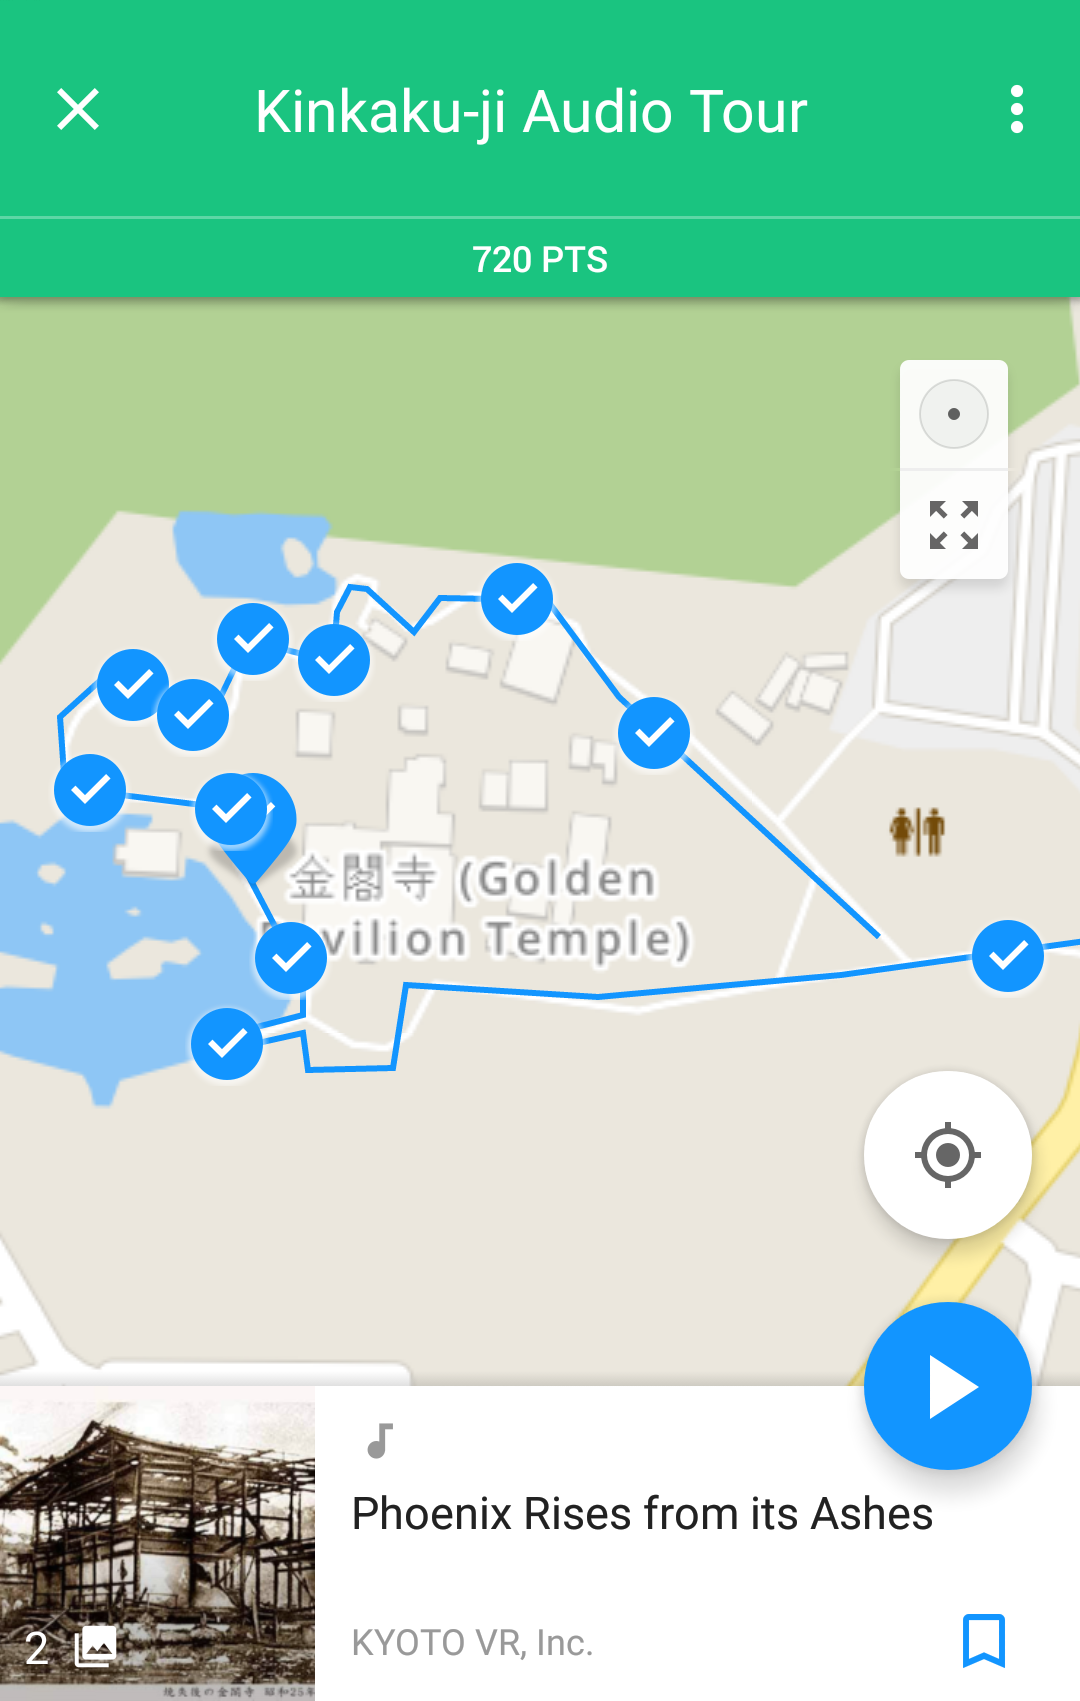
\includegraphics[width=.5\textwidth]{izi-travel.png}
	\caption{A screenshot of the izi.TRAVEL app interface}
	\label{fig:iziTravel}
\end{figure}

\begin{figure}[h]
	\centering
	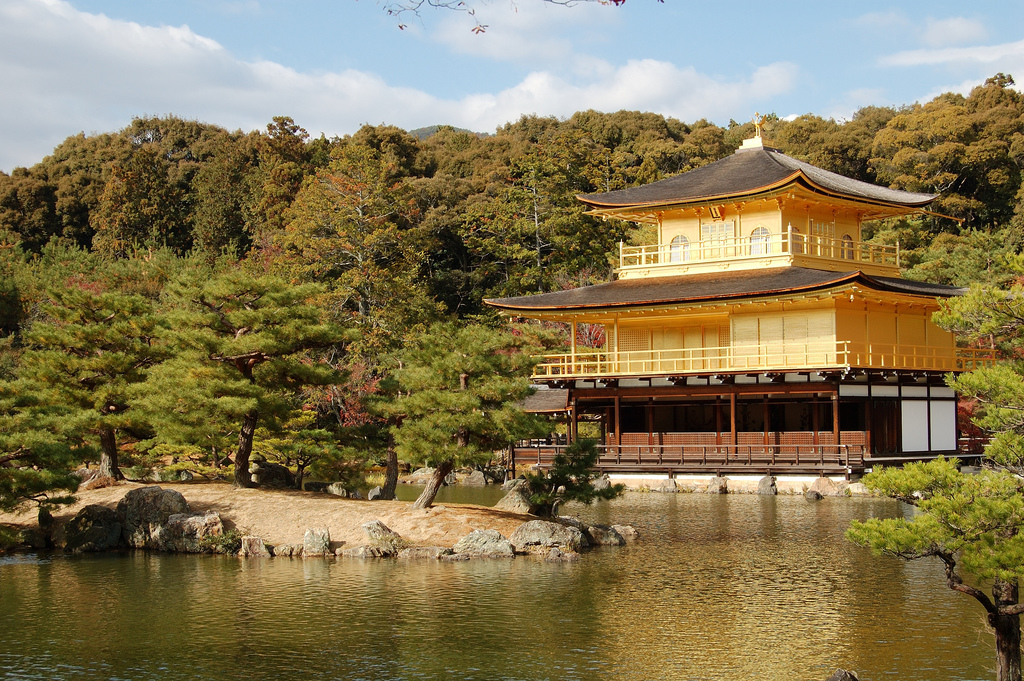
\includegraphics[width=\textwidth]{kinkakuji.jpg}
	\caption[The Golden Pavilion of Kinkaku-ji, Kyoto, Japan]{The Golden
		Pavilion of Kinkaku-ji, Kyoto, Japan~\autocite{davidson2005}}
	\label{fig:kinkakuji}
\end{figure}

By using GPS data from the user's phone to play audio and display images at
specific places in the real world izi.TRAVEL uses a limited form of augmented
reality. Our group aimed to implement and extend this functionality in our own
app. See Section \ref{sec:aruko} for more details.

\subsection{Platforms}
\label{sec:platforms}

Before we could start working on creating our app, we first needed to decide which
AR development platform to use. Our preliminary research had shown us that there
are so many different platforms out there, all of which have been used to create
great AR apps. There were a lot of things we needed to consider before finalizing
on a platform, like what features it offered, which devices and operating systems the
app could run on, and definitely the cost. Detailed below are some of the different
platforms we considered.

\subsubsection{ARCore and ARKit}
\label{sec:ARCoreAndARKit}

ARKit and ARCore are both AR frameworks that enable apps to take advantage of
powerful AR related features. ARKit is developed by Apple and can only be used
by iPhones. Google's ARCore framework can deploy to both Android and iPhone.
Many cross platform solutions will leverage the full potential of their target
platform by using either ARKit or ARCore ``under the hood''. Both ViroReact and
Vuforia use ARKit or ARCore depending on the target platform
\autocites{vuforiaFusion}{moon2018}.

ARKit 3 aims to support a wide array of new features and will be available in
iOS 13. Notably, one of these features is ``people occlusion,'' which will allow
virtual objects to be realistically obscured when someone walks in front of the
object~\autocite{apple2019}. This kind of technology could be useful for us
since our app uses AR in crowded places.  As of August 2019, this feature is
not on the horizon for Google's Android AR framework, ARCore.

Both ARKit and ARCore have well-supported APIs for Unity. ARKit 3 support is
coming to Unity, along with all of the advanced features that it
brings~\autocite{stinson2019}.

\subsubsection{Wikitude}
\label{sec:wikitude}

Wikitude is another major AR development kit that is very prevalent in the
world of AR development. It has over 130,000 registered AR developers, and is
powering over 30,000 AR apps across smartphones, tablets, and smart
glasses~\autocite{wikitude2018}.  And it's easy to understand why Wikitude has
so many registered developers when you see the list of features it offers. Some
of the features that appealed most to us were their Instant Tracking, allowing
for augmentation using flat surfaces; Image Tracking, allowing for augmentation
using one or multiple 2D images; and Geo AR, allowing for creation of geo
markers at specific locations to triggered AR content~\autocite{wikitude2018}. 

Wikitude also supports all sorts of different platforms. It supports Android, Apple,
and Windows phones and tablets, as well as smart glasses like the Epson Moverio,
Microsoft Hololens, and Vuzix smart glasses~\autocite{wikitude2018}. Additionally,
many different development frameworks are capable of running Wikitude's SDK.
According to Wikitude's website, their SDK works with Windows, Android, and iOS
development frameworks, as well as ARCore and ARKit, Flutter, Cordova, Xamarin,
and even Unity~\autocite{wikitude2018}. 

From all of this information, Wikitude certainly sounds like a fantastic AR
development platform; it certainly did to us. But the issue we ran into was the
cost. Wikitude is, in fact, free for eligible startups, but given the criteria
they list on their site, we were not confident that we would qualify. Aside
from this option, Wikitude offers a 30-day demo license for \euro{499}, which
is a lot for use to pay for a license that would not even last for our entire
project. They also charge \euro{1990} for their SDK Pro, and \euro{2490} for
their SDK Pro 3D~\autocite{wikitude2018}. Given these prices, and our very
limited budget, we knew that we would have to pass on Wikitude and choose a
different AR development platform. 

\subsubsection{motive.io}
\label{sec:motive.io}

The company motive.io used to work on a product that would allow users to
create an engaging AR experience in the style of Pokemon Go. Their service
would have purportedly handled technical details such as hosting, storage, and
user accounts. The promotional video shows the creation of a location-based AR
game where the user pretends to hack into ATMs using the real-world locations
of ATMs in a city\autocite{odom2017}.

Unfortunately, it appears that the company has completely pivoted off of this
idea, and has since moved to AR training software\autocite{motiveio}.

We reached out to motive.io via email for any advice they might be willing to
give us, but we received no response.

\subsubsection{Viro AR}
\label{sec:viroAR}

Viro AR comes in two flavors: ViroReact and ViroCore. ViroCore allows
developers to build an AR Application with Java. The disadvantage of this is
that ViroCore only allows developers to target Android, which unfortunately
made ViroCore not an option for our project. ViroReact is the cross-platform
option for ViroAR. ViroReact leverages the cross-platform capabilities of
React, which is Facebook's Javascript Library for developing user
interfaces~\autocite{facebook2019}.

Since our project is not a game, we initially wanted to avoid using a
fully-featured game engine. Therefore, we decided to take the time to explore
this framework since it appeared to be more tailored to our specific use case.
Viro Media also recognizes that all developers who wish to create an app with
3D capabilities are not necessarily game developers. Viro Media pitches Viro
AR as ``The perfect alternative to specialized game engines, ViroAR is a
platform for rapidly building ARKit and ARCore apps. Our platform allows
developers to focus on what they do best by leveraging familiar tools and
frameworks used in mobile application development''~\autocite{viro2019}.
While the majority of our team has decent experience with writing Javascript,
we all either have very little or no experience writing React apps.

In most development scenarios, every time you wish to test your app on actual
hardware, you must first compile your app using either Xcode or Android Studio
depending on your platform. Once you have built the app, your device needs to
install the app. This process can be very time consuming, especially since
frequent tests on real hardware is important for something as intensive as
AR.

An alternative to building your app is to run your app through an emulator on
the computer you are using for development.

According to Techopedia, ``Emulation is the process of imitating a
hardware/software program/platform on another program or platform. This makes
it possible to run programs on systems not designed for
them''~\autocite{techopedia2019}. Emulators are often very useful for speeding
up development. Loading programs onto the Android emulator usually much faster
than installing the APK onto the actual device. Additionally, you can mock
almost all of the important features of an actual Android device, including
calls, text, GPS position, device rotation and more \autocite{androidemulator}.

Since an emulator uses software to emulate hardware, this poses two technical
issues that prevent emulators from being a proper replacement for testing on
real hardware.  Emulation is often imperfect, so glitches sometimes emerge in
emulation that do not manifest on the actual hardware [citation needed about
emulator inaccuracies]. Conversely, errors that exist in the hardware version
may not appear in the emulation. Secondly, and most importantly for AR, it is
common for emulation to be much slower compared to real hardware.

In a question submitted to \textit{Compute!} magazine asking whether it is
possible for a Commodore 64 to emulate MS-DOS, the editor responded ``Yes, it's
possible for a 64 to emulate an IBM PC, in the same sense that it's possible to
bail out Lake Michigan with a teaspoon.'' The editor goes on to explain
``Emulation is a complex business, but here's one rule of thumb: The only way to
successfully emulate a machine is with a much more powerful
machine''~\autocite{warick1988}. In our case, emulating Android on a desktop
operating system is closer to emulating a C64 on an IBM PC running MS-DOS
(rather than the other way around, thankfully). The moral is that the speed
problem facing emulators is just as real as it was in 1988. Considering that AR
already pushes modern phone harware to the limit, emulation is not something is
not something we wanted to struggle with. On top of this, our testing required
us to move the camera through the world at various speeds and angles, which is
simply cumbersome with a laptop webcam.

As an alternative to emulation, ViroReact offers a convenient ``test bed'' for
rapidly testing your ViroReact app on native hardware without the need for an
emulator. In the root directory of your project, you can launch a Node server
with the command \texttt{npm start}. From here, you can input the provided URL
into the Viro Media app. This will quickly download the code, graphics, and 3D
object files from the server and launch a functional version of the app
\autocite{viro-testbed2019}. This allowed us to get a real AR app up and
running on our devices much more easily than any of the other
frameworks/engines we explored. Unfortunately, the test bed app was somewhat
unreliable based on our experience; the test bed would frequently crash or
would not be able to download the files from the Node server. The most reliable
way to test our app was to compile a binary and manually install it onto our
devices, which completely defeats the purpose of the test bed app.

\subsubsection{Unity}
\label{sec:unity}

\subsection{Kinkaku-ji}
\label{sec:kinkaku-ji}

We were tasked with building an AR mobile app that enhances the experience of
visiting Kinkaku-ji, also known as the Golden Pavilion. As of September 2019,
Kinkaku-ji is the second-most visited site in Kyoto---second only to Kyoto
Station \autocite{japanguide2019}.

\newpage

\section{Implementation and Technology}
\label{sec:implementationAndTechnology}

\subsection{Editour: The Tour Editor}
\label{sec:editour}

The goal of Editour is to allow a non-technical user to design audio tours
through a web-app. At its core, Editour is a tool to draw arbitarily-shaped
geographic regions onto a map. 

An audio file and multiple image files can be uploaded for each region the user
defines. The user can also provide a text transcript of the audio file as well.
After naming and uploading the tour with the ``Upload'' button, our backend
builds a zip containing a folder that can be placed directly into the Unity
project.

Our backend allows users to save their tours to our server and load those same
tours back into the editor to resume work.  The geographic area of each region
can be adjusted by clicking and dragging. Vertices can also be added and
deleted if the needs of the tour change over time.

\subsubsection{The Need for an Editor}

One of the goals for our project is to create a working prototype that others
can build off of in the future [citation needed for personal communication].

Similar to the app izi.TRAVEL discussed in section~\ref{sec:iziTravel}, we
needed some way to easily define arbitrary polygons (which we call ``regions'')
and associate media with each one, such as audio and image files.

For testing purposes, we initially defined these regions directly in the C\#
Scripts, hard-coding the coordinates. [citation needed for source used to
write polygon detection code] Below is an example of a quadrilateral
surrounding the Creation Core building at the Ritsumeikan Biwako-Kusatsu
campus.

\begin{minted}{csharp}
Regions.add(new GPSPolygon(new List<GPSPoint>{
    new GPSPoint(34.979222, 135.963628),
    new GPSPoint(34.979187, 135.965130),
    new GPSPoint(34.979794, 135.965053),
    new GPSPoint(34.979754, 135.963669)
}, "Creation Core"));
\end{minted}

Even with knowledge of C\# and Unity, inputing tour data this way is obviously
not convenient. Atticus reminded us that, although he has a working knowledge
of Unity, he is not a software developer [citation needed for personal
communication.] In order to make our app prototype at all useful for the
future, we needed to provide an easy way to ``design'' a tour.

\subsubsection{A Complete Tour Definition}
\label{sec:tourDefinition}

In order to create a fully-functional editor for designing and exporting
``tours,'' we had to consider how to fully define a tour purely in terms
of text and a directory of associated media.

Here is an example of the JSON metadata generated by Editour:

\begin{minted}{json}
{
   "regions": [
      {
         "name": "Beautiful Place",
         "points": [ {"lat": 23.4, "lng": 56.7}, /* list omitted for brevity */ ],
         "audio": [ "beautiful-audio.mp3" ],
         "images": [ "mountain.jpg", "stream.jpg" ],
         "transcript": "To your left, you can see a beautiful place."
      },
      {
         "name": "Gorgeous Place",
         "points": [ {"lat": 12.3, "lng": 45.6}, /* list omitted for brevity */ ],
         "audio": [ "gorgeous-audio.mp3" ],
         "images": [ "hill.jpg", "valley.jpg", "gorge.jpg" ],
         "transcript", "To your right, you can see a gorgeous place."
      }
   ]
}
\end{minted}

Within each object in the region list, we can see that the region has five
properties: a name, a list of coordinates, a list of audio files, a list of
multiple image files, and a transcript of the audio file. (In the current
design of the app, it only makes sense to associate one audio file per region,
but the format makes it easy to accommodate for multiple audio files in the
future.) One disadvantage is that all media files have to have unique names.
This is because the zip that is created by the Editour backend contains all of
the media files in a flat file structure. The above JSON is used to associate
each media file with a region, meaning that the filename needs to act as a
primary key. The backend will respond with a message if this is the case,
prompting the user to have unique names for all files.

\subsubsection{Editing a Tour}
\label{sec:editingATour}

The user can easily create a new region by shift-clicking, and then clicking
points on the map.  To terminate the polygon, the user must shift-click again.
The ``Welcome to Editour'' card (seen in Figure~\ref{fig:welcomeCard}) provides
these instructions, which should be enough to get started.  A user can only
terminate the polygon after two points have been placed to prevent the user
from drawing a region with an area of zero. Once a region is created, a region
card appears in the side bar. From here, the user can edit anything about the
region. From here, the user can edit anything about the region.

\begin{figure}[h]
	\centering
	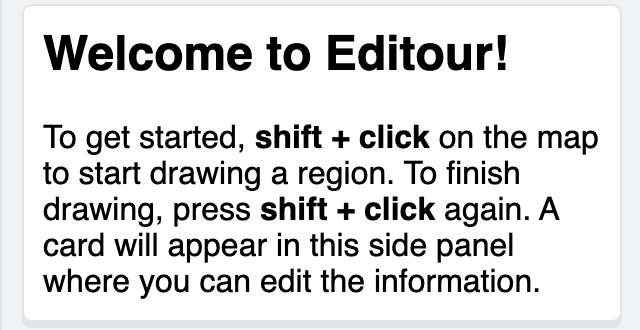
\includegraphics[width=0.4\textwidth]{welcome-card-editour.png}
    \caption{The ``Welcome to Editour'' card providing basic instructions to
    get started}
	\label{fig:welcomeCard}
\end{figure}

\begin{figure}[h]
	\centering
	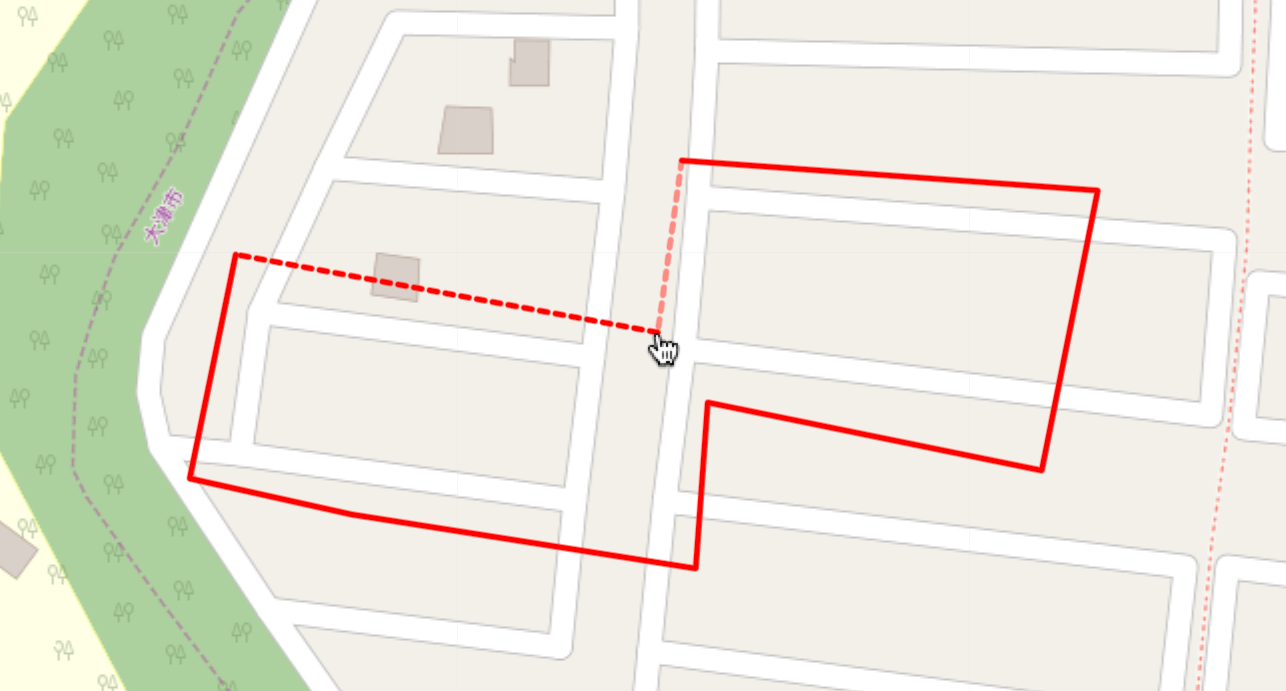
\includegraphics[width=0.5\textwidth]{drawing-region-editour.png}
    \caption{How the Editour looks when a region is being drawn, including the
    two dotted preview lines}
	\label{fig:drawingRegion}
\end{figure}


The top of the region card displays the region name in bold text. By clicking
on the region name, the map will pan and zoom to frame the region in the center
of the screen. This is useful if there are many regions. To the right of the
region name, there are two arrow buttons, one pointed up and another pointed
down. This allows the user to reorder the regions in the column. This was one
of the features that was added late into development in order to adapt to an
important change in the tour app, ARuko. This is discussed in
Section~\ref{sec:adobeXdDesign}.

In the region card, there are four multicolored expandable ``subcards'' that
allow the user to edit different information about each region. Since there can
be many region cards in the column, it was important to be able to collapse
each section. Collapsing the subcards gives the user enough room to see
multiple region cards at a time.

The first subcard seen in Figure~\ref{fig:renameSubcard} is the ``Rename''
subcard, which is fairly self-explanatory.  This section expands to reveal a
textbox, allowing the user to rename the region after clicking ``Okay'' or
hitting the enter key. (There are multiple places in the UI where a textbox is
immediately adjacent to a ``Confirm'' button.  We made sure all of these can be
triggered by simply hitting enter, since this is common when filling out
forms.)

\begin{figure}[h]
	\centering
	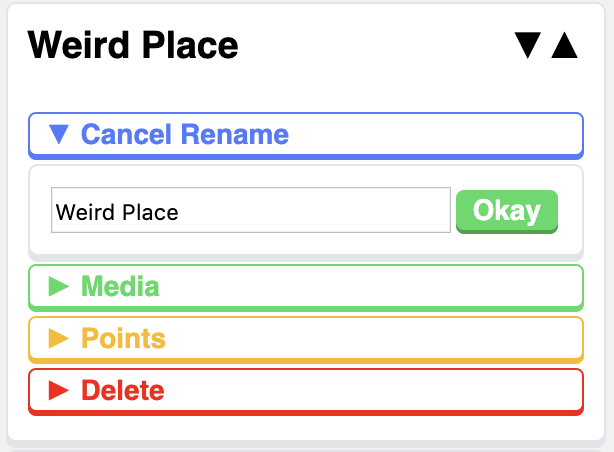
\includegraphics[width=0.4\textwidth]{rename-subcard-editour.png}
	\caption{The ``Rename'' subcard}
	\label{fig:renameSubcard}
\end{figure}

The second subcard seen in Figure~\ref{fig:mediaSubcard} is slightly involved.
Expanding the ``Media'' subcard by clicking on the green bar will reveal a bevy
of options for augmenting the audio, images and text to be associated with that
region of the tour. From here, the user can upload an audio file and multiple
image files from his or her hard drive with the two file-select fields. If the
tour has been downloaded as a server, the names of the files already present on
the server will appear as cards with `X' buttons. This allows the user to
remove images or audio from that region even after the tour has been uploaded.

\begin{figure}[h]
	\centering
	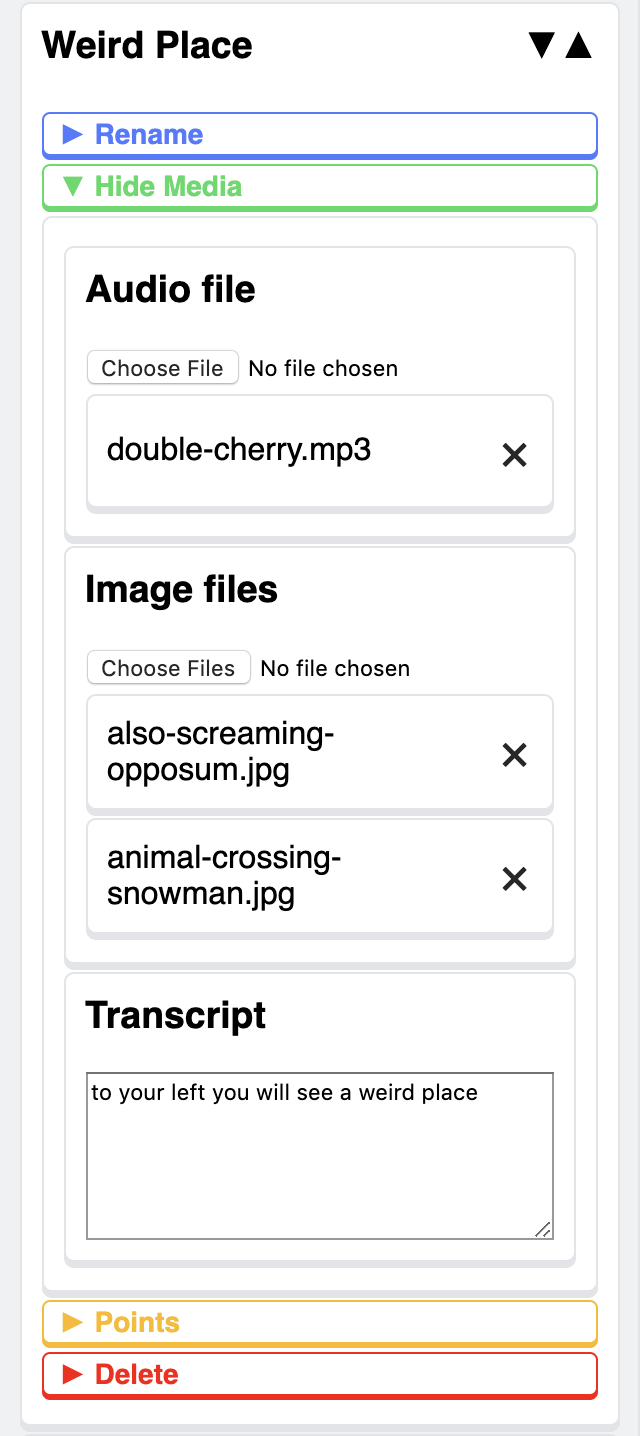
\includegraphics[width=0.4\textwidth]{media-subcard-editour.png}
	\caption{The ``Media'' subcard}
	\label{fig:mediaSubcard}
\end{figure}

The third subcard is the ``Edit'' subcard. This subcard can be revealed in one
of two ways. The first way is by clicking on the yellow bar labeled ``Edit'',
which is the same for all subcards. Alternatively, the user can also click
directly on the region on the map. The region will flash yellow and be scrolled
into view to let the user know which region was clicked on. Both of these
methods will enable editing mode, whereby the user can directly manipulate the
vertices that make up the region. Blue circles appear on top of each vertex,
and red circles appear at the midpoint of each edge. Clicking on a red midpoint
will add an additional vertex at that midpoint. Dragging one of the blue
vertices will do as you might expect---move the vertex around. The latitude and
longitude are updated in the ``Edit'' subcard as the user drags the vertex
around. Clicking on the vertex directly will create a blue pin-shaped marker
that the user can also drag around. Clicking on the coordinate box in the
subcard will also create this blue pin-shaped marker; the map will also pan to
this coordinate. The user can also delete vertices in the same way that files
can be deleted from the ``Media'' subcard by clicking on the `X' button. If there
are exactly three points in a region, the `X' buttons will be ``grayed-out'',
preventing the user from deleting any more points (since a polygon must consist
of at least three points.)

\begin{figure}[h]
	\centering
    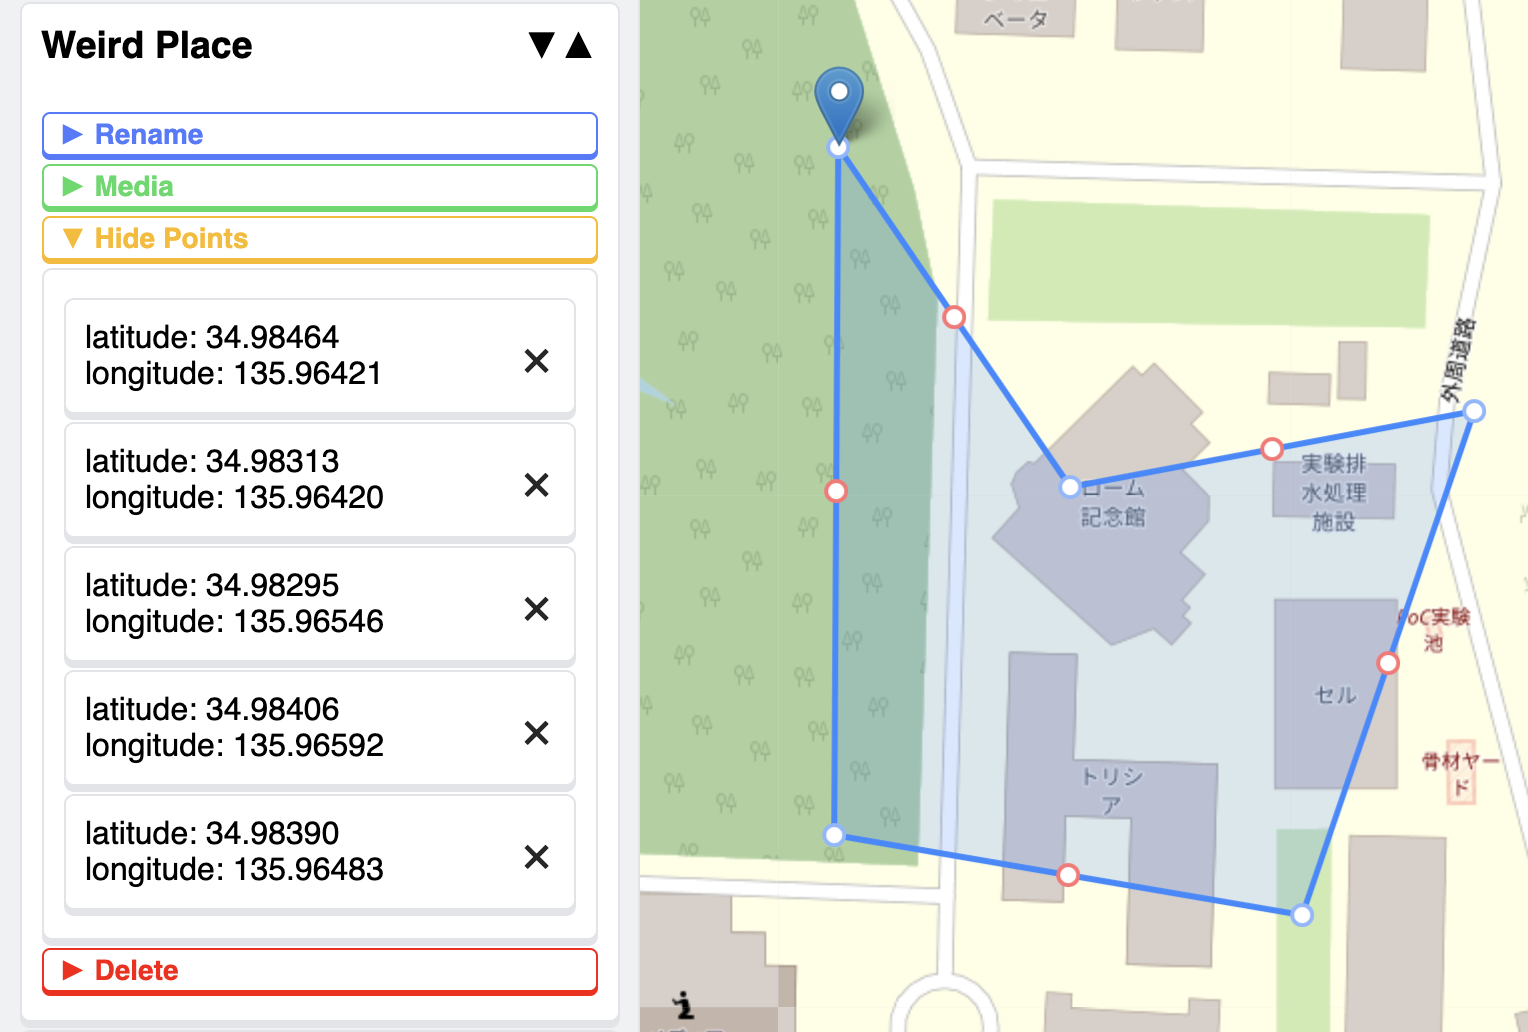
\includegraphics[width=\textwidth]{edit-subcard-with-map-editour.png}
    \caption{The ``Edit'' subcard with the map showing vertices and edges that
    can be edited}
	\label{fig:editSubcardWithMap}
\end{figure}

The third subcard pictured in Figure~\ref{fig:deleteSubcard} is the ``Delete''
subcard. When revealed, another button will appear labeled ``Really Delete''.
The action can be canceled by collapsing the subcard by hitting the bar now
labeled ``Don't Delete!''. This prevents the user from accidentally deleting a
region he or she did not mean to.

\begin{figure}[h]
	\centering
    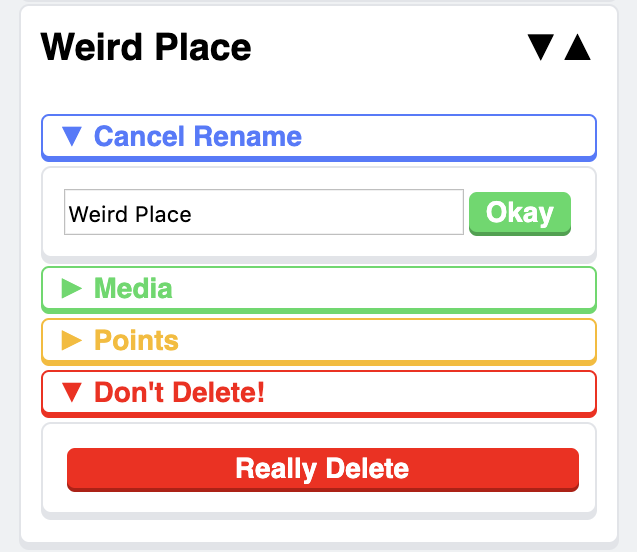
\includegraphics[width=0.4\textwidth]{delete-subcard-editour.png}
    \caption{The ``Delete'' subcard}
	\label{fig:deleteSubcard}
\end{figure}

Above all of the region cards, there are various options for uploading,
downloading, renaming and deleting tour files on the server. Within the upload,
download and delete cards there are message boxes to indicate the status of
that operation. When uploading and downloading, a percentage will be displayed
indicating the upload/download process, which can be seen in
Figure~\ref{fig:uploadingMessage}. If a 200 or 201 is returned from the server,
a ``Success'' message will appear. If there was some problem, the error message
returned by the server is displayed in this box instead. Since uploading,
downloading and deleting are all network-related operations, it makes sense to
include this message box for each card.

\begin{figure}[h]
	\centering
    
\includegraphics[width=0.4\textwidth]{uploading-message-editour.png}
    \caption{The upload subcard with an upload status}
	\label{fig:uploadingMessage}
\end{figure}

When the page is loaded, the frontend will request the names of the files
stored on the server from the backend. This data is used to create a box of
buttons, which includes one button for each tour file on the server. Clicking
on one of these blue buttons will fill the textbox in with the correct name.
Before this feature was implemented, the user had to correctly type the name of
the saved tour into the textbox in order to retrieve it. The user is still free
to do this, but the buttons make this easier and less error-prone. The download
card containing a box filled with filenames on the server can be seen in
Figure~\ref{fig:downloadCard}.

\begin{figure}[h]
	\centering
    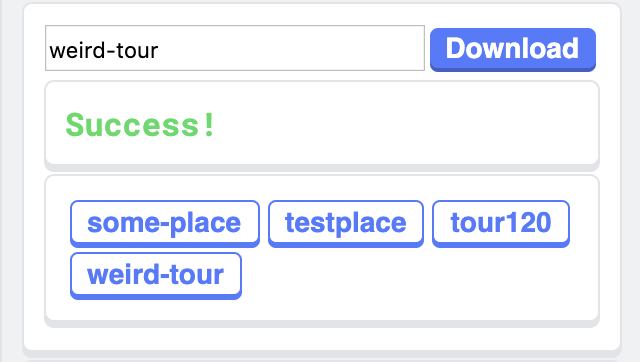
\includegraphics[width=0.4\textwidth]{download-card-editour.png}
    \caption{The download card}
	\label{fig:downloadCard}
\end{figure}

We did not include a way to resolve addresses or place names, like the service
provided by Google Maps. Instead of exploring plugins/libraries that might
provide this functionality, we offered a simpler solution due to time
constraints.  You can type in a latitude and longitude directly and hit the
``Jump'' button. We also hard-coded a few shortcuts for places that Atticus
might want to design a tour for in the future, which can be accessed by
clicking on the yellow buttons with place names.

\begin{figure}[h]
	\centering
    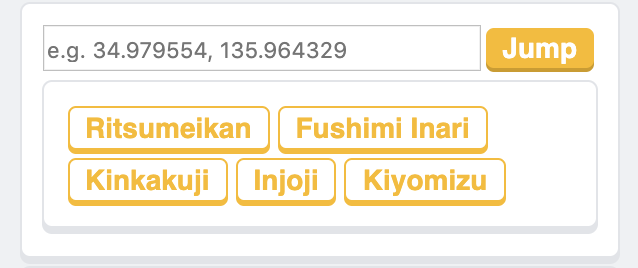
\includegraphics[width=0.4\textwidth]{jump-card-editour.png}
    \caption{The jump card}
	\label{fig:jumpCard}
\end{figure}

Once a tour is either uploaded or downloaded, a link to download the zip file
will appear. The zip file contains all of the uploaded media, and a metadata
file. The metadata is in the form of a JSON file; it contains all of the
latitudes, longitudes, and enough information to associate all of the media
with the correct regions. This is the file that we unzip and place into the
Unity project before it is compiled. This also is useful if the user wants to
check the audio and image files that were uploaded.

\begin{figure}[h]
	\centering
	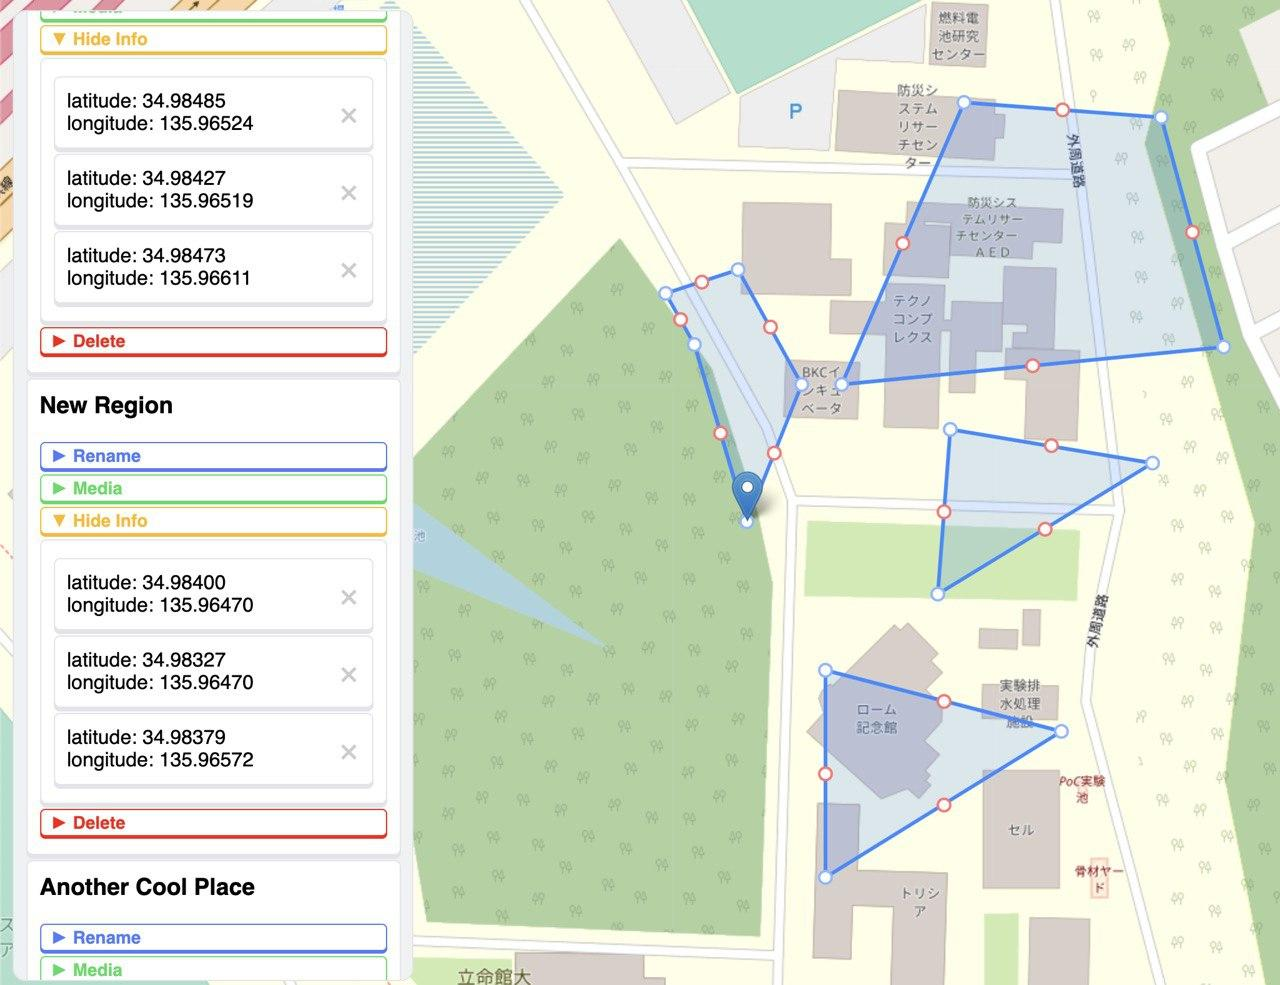
\includegraphics[width=\textwidth]{editour.jpg}
	\caption{A screenshot of the Editour web app frontend}
	\label{fig:editour}
\end{figure}

\subsubsection{Editour Backend}
\label{sec:editourBackend}

The server-side backend of the Editour application is written in JavaScript for
Node.js. This backend both serves the static frontend content and runs
server-side scripts that process incoming API requests.  We chose Node.js as the
server-side framework because of our prior experience with JavaScript, its
high-performing asynchronous architecture~\autocite{orsini2013}, and its ease of
development.

When a user submits new tour from the web application, the files and metadata
are sent to the server running the Node.js scripts, which zips up the files and
saves them to the server's disk with a timestamp. Then any application can
request a particular tour and the backend will serve the most recent version of
it.

As previously mentioned in \ref{sec:editingATour}, our web application allows
users to edit existing tours. When the user requests to edit a tour on the
frontend it sends a request to the backend server for that tour's metadata
file. This file contains information about all regions and files in the tour.
The user can then edit the regions, change names, upload new files, or delete
existing ones without ever having to download the other tour files from the
server, which could take a long time depending on their size. When the user is
done editing they can upload the new metadata and any newly added files to the
server, which intelligently collects new and old files required by the tour and
zips them into a new tour file on the disk.

\subsubsection{Future of Editour}
\label{sec:futureOfEditour}

In the current implementation, the tour file generated by the Editour backend
still has to be moved manually to the Unity project folder. In the future, we
would like the app to be able to contact our Editour server and update the tour
info by itself. This would allow Kyoto VR to update the tours without updating
the entire app.

The design of the Editour is agnostic about how the media will be used. For an
app like izi.TRAVEL, the images are displayed when the associated audio tour is
playing. The tour files produced by Editour could theoretically be used by a
tour guide app that does not incorporate AR. 

\subsection{ARuko}
\label{sec:aruko}

\subsubsection{Adobe XD Design}
\label{sec:adobeXdDesign}
On September 10th, Atticus Sims presented us with a storyboard for the app
experience. We would not be able to resume work until September 17th due to
prior travel plans. Whether Atticus knew this or not, the design he put forth
had ramifications that rippled throughout the entire software stack we had
constructed up to this point. Figure~\ref{fig:adobeXdDesign} shows this design.

\begin{figure}[h]
	\centering
	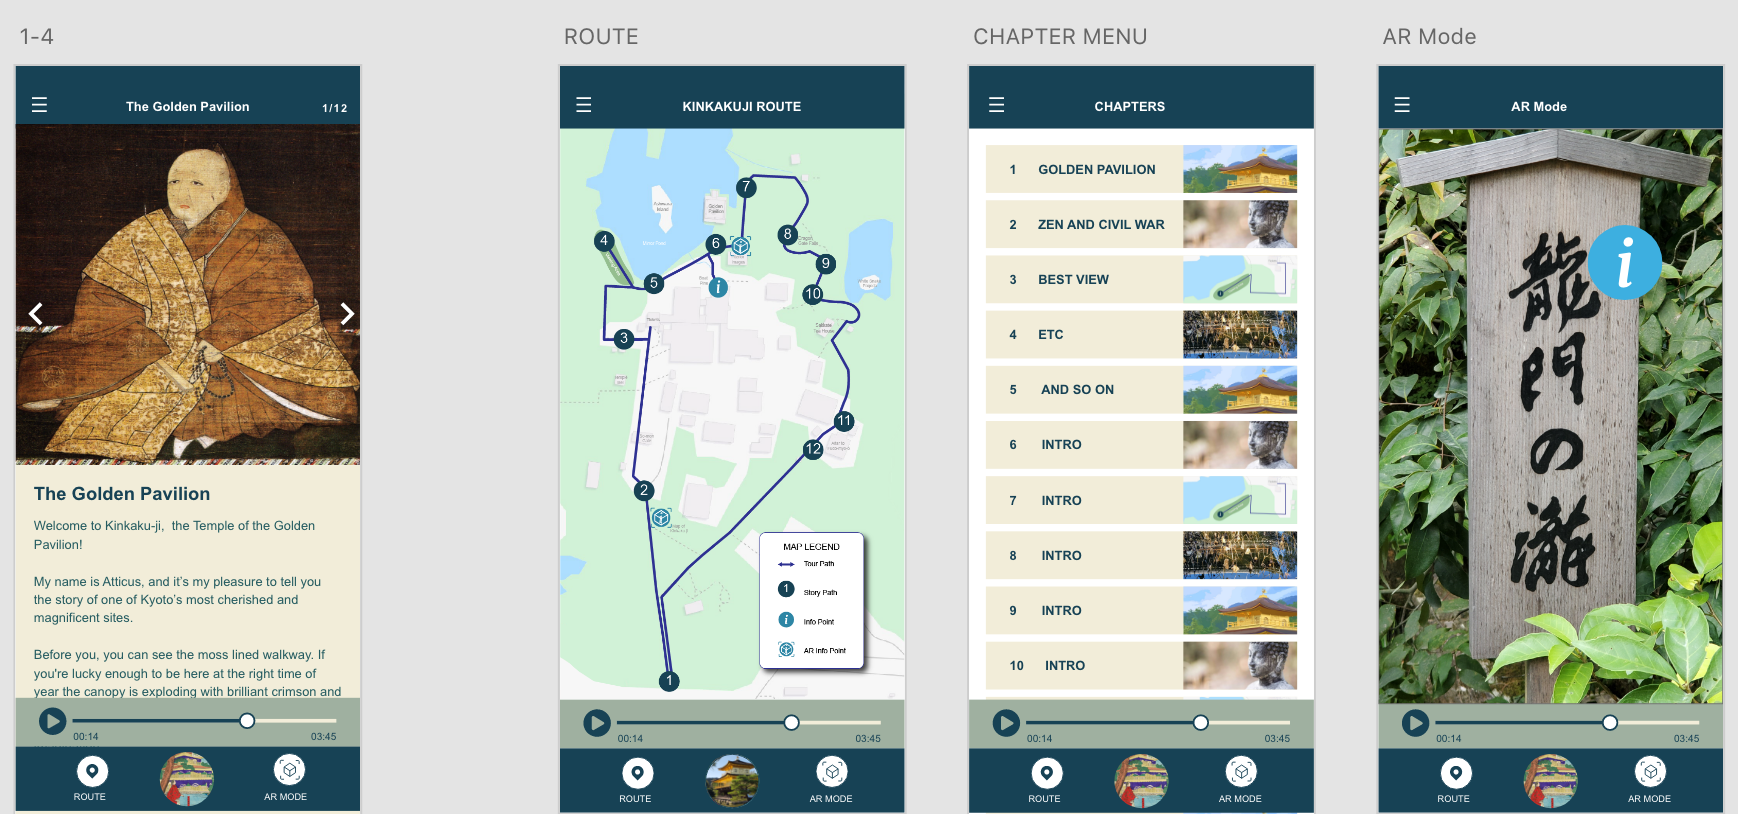
\includegraphics[width=1\textwidth]{adobe-xd-design.png}
	\caption[A screenshot of the Adobe XD project designed by Atticus Sims]
    {A screenshot of the Adobe XD project designed by Atticus Sims}
	\label{fig:adobeXdDesign}
\end{figure}

One of the notable changes is the chapter select screen, which is the third
screen in Figure~\ref{fig:adobeXdDesign}. Before, we worked under the assumption
that each geolocation-triggered region would not have to be ordered in any way.
This assumption made its way into Editour, which did not currently have a way
to reorder regions once they were placed. Because of this chapter selection
screen, we needed some way to rearrange the order of regions within Editour.

Another notable change can be seen in the first screen on
Figure~\ref{fig:adobeXdDesign}. Atticus was not enthusiastic about being able
to place images onto the ground-plane using the AR camera. Instead, he
suggested that we have the images be viewable in a more traditional
fashion---in 2D as part of the UI. This was disappointing to us, since we spent
a great deal of effort projecting images into the 3D world using the AR camera;
we felt like we figured out how to use this technology in a way that was both
usable and fun. Ideally, we wanted to explore ways to theme the 2D images in
the 3D world, such as by framing the images in a traditional Japanese pagoda,
which would fit in with the environment. On the same screen, there is a
scrollable window of text for a transcript of the audio. Because of this, the
Editour UI and tour metadata JSON file needed to be updated to accomodate a
transcript per region. On top of this, the C\# code that interprets the tour
file needed to be updated to expect an audio transcript field.
Figure~\ref{fig:editourAdditions} shows the UI elements that changed in order
to add these new features. The arrows next to the region name can be used to
move the ``Region Card'' up and down in the side bar. In the ``Media'' tab, there
is also a text area to include a transcript of the uploaded audio file. 

\begin{figure}[h]
	\centering
	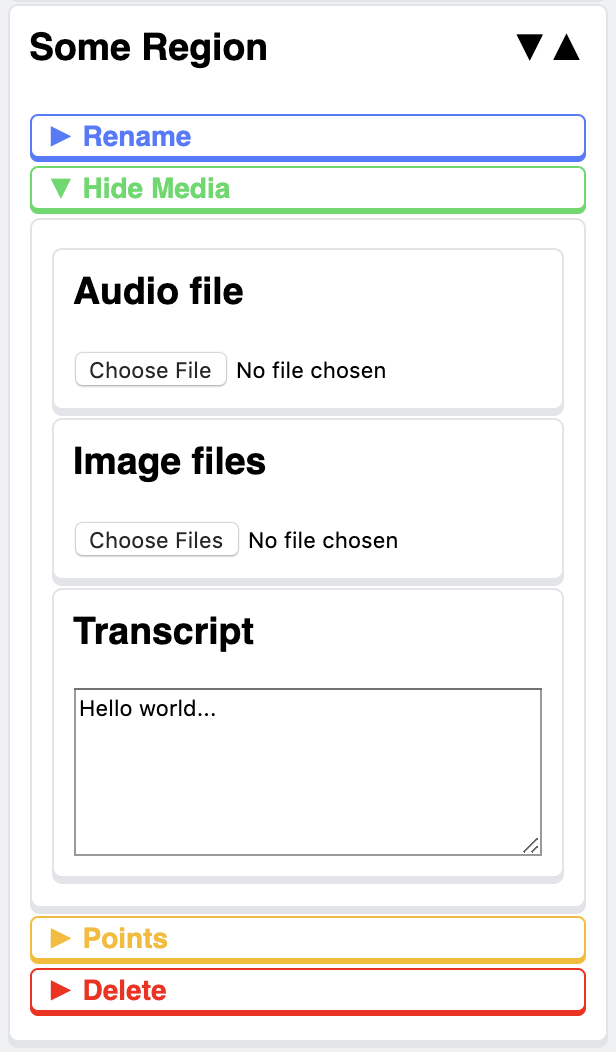
\includegraphics[width=0.5\textwidth]{editour-additions.png}
	\caption[Additions to the editour to accommodate the new design]
    {Additions to the editour to accommodate the new design}
	\label{fig:editourAdditions}
\end{figure}

At this point, the codebase for Editour was already around three thousand lines
of vanilla Javascript. Type-checking provided by Visual Studio Code and JSDoc
made the growing code complexity more manageable. Excluding Node.js modules,
the only external library we used for Editour was Leaflet, an open-source
JavaScript library for interactive maps \autocite{leafletjs}. We did not use
any libraries for developing frontends like Facebook's React or Google's
Angular. Instead, all of the complex UI interactions were handled by modifying
the DOM directly with JavaScript's built-in functionality. Furthermore, we did
not use any advanced frontend build tools such as Rollup, webpack or Parcel.
This was likely an appropriate decision for a JavaScript project of this scope.
Considering we had limited to no experience with React or Angular, it was also
faster to develop the UI in the way we were used to from previous experience..
But if we were to continue to develop Editour, UI libraries and frontend build
tools would be something to consider. With these changing requirements, the
Editour was becoming onerous to maintain at this stage of the project.

With the ground-plane detection features stripped away from the main app, the
AR focus shifted to translating the maps and signs using the camera. The fourth
screen on Figure~\ref{fig:adobeXdDesign} shows a mock-up of this feature.
Atticus took photographs of various signs throughout Kinkaku-ji for us to use as
image targets. Hikaru Inoue helped us by translating all of the text in these
photos from Japanese to English. In this design, the AR camera superimposes an
``info'' button on top of the sign. Tapping on this button brings up a separate
UI element containing the translation, which can be seen in
Figure~\ref{fig:signTranslation}.

\begin{figure}[h] \centering
    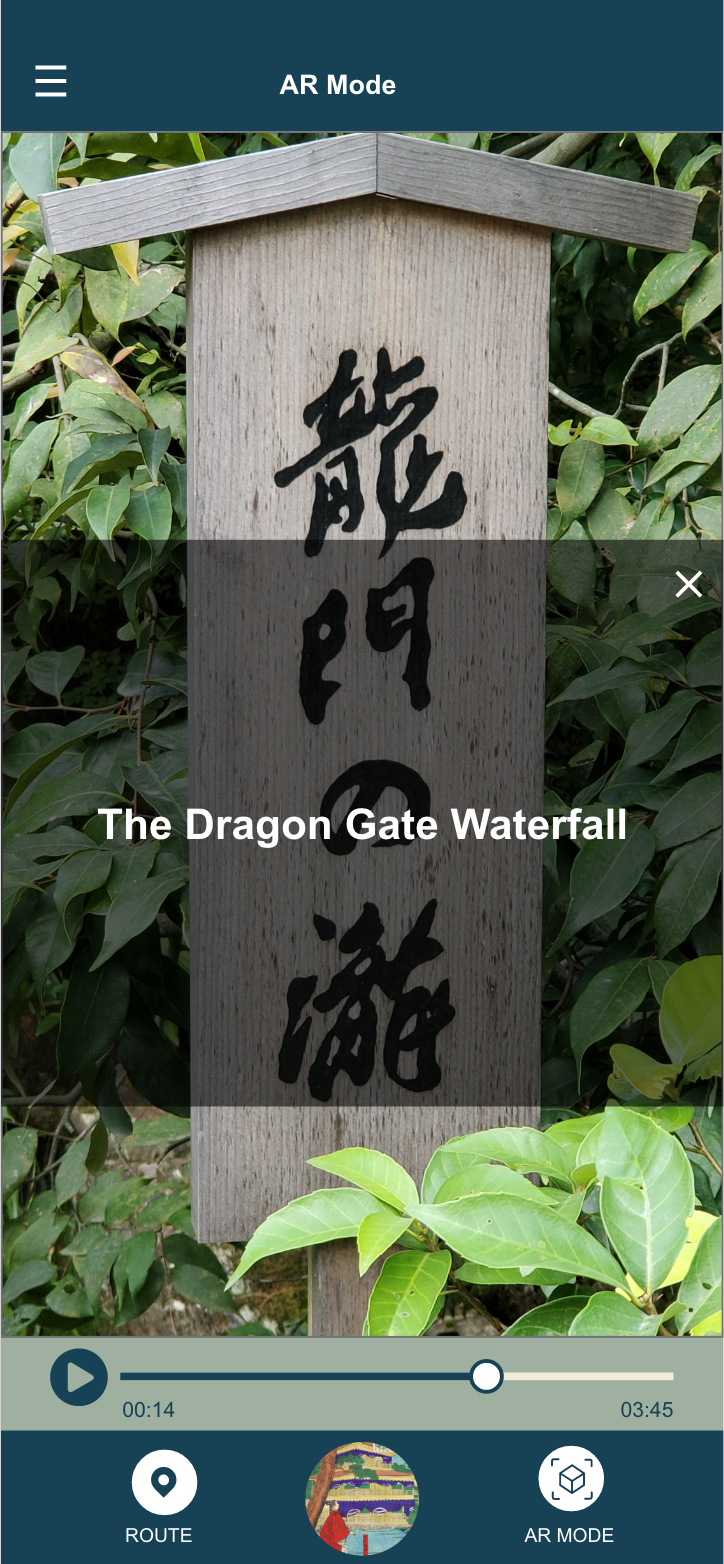
\includegraphics[width=0.5\textwidth]{sign-translation.png}
    \caption{Translated sign using AR camera}
    \label{fig:signTranslation}
\end{figure}

As previously mentioned, Atticus initially wanted us to explore the efficacy of
using Vuforia's 2D image target capabilities for scanning objects outside of
the expected use case, such as 3D landscapes or the side of a building. We had
serious doubts about how well this would work, and our suspicions were
confirmed after some field testing. This was the reasoning behind focusing on
ground-plane detection instead of image targets; ground-plane detection can be
used anywhere, and is much more reliable than treating 3D objects as 2D image
targets.

Since Adobe XD is largely a prototyping and design tool, a considerable amount
of legwork would still need to be done to rebuild the proposed design using
Unity's UI components. Adobe XD allowed us to export a few important UI
elements as PNGs, such as the buttons to enter AR mode and view the map. We
briefly explored a few solutions to automating the task of getting the Adobe XD
project into Unity. We found one payed extension (for \$18) on the Unity Asset
store, called ``Experience Importer - Adobe Xd files importer'', which claims
``Transfer AdobeXd project directly to Unity. Forget about hours of positioning
objects. They're already there! Just drag .xd file to project and... voila!''
We suspect this sounds too good to be true because it is. As of September 20th,
2019, there are 6 user reviews. All of the five-star reviews were have the
caveat ``Reviewer was gifted package by publisher'' which which we interpreted
as a warning sign. Because of this, we decided to rebuild the UI largely from
the ground up, using the Adobe XD file to guide us.

\newpage

\section{Testing}
\label{sec:testing}

Both pieces of our project---the Editour and ARuko---are designed to be used by
people who aren't programmers. The Editour will be used by Atticus in the future
to design more tours, and ARuko will be used by the general public. Because of
this, we needed to do extensive testing to ensure not only that the products
work as intended without bugs, but also that they would be pleasant and easy to
use for their intended users.

\subsection{Testing Editour}
\label{sec:testingEditour}

Because the Editour is intended only to be a tool to aid Atticus in creating
tours, not an application for the general public, our user testing of it was less
rigid.

\subsubsection{Unit Testing the Editour Backend}
\label{sec:unitTestingTheEditourBackend}

To test the API and backend of the Editour web app we used the Mocha testing
framework. Mocha is the most depended-upon package in the Node Package
Manager~\autocite{tidelift2019}, and is widely used by professional software
development teams. It has a myriad of useful features that allow developers to
quickly write unit tests for complex Node.js projects~\autocite{mochajs2019}.
Most importantly for us, it has good support for testing asynchronous JavaScript
functions, since most of the backend is written asynchronously. Along with Mocha
we also used SuperTest, a library for writing high-level end-to-end HTTP
tests~\autocite{supertest2019}.

For each of the six API endpoints that the backend responds to we wrote an
extensive series of end-to-end tests to ensure that each step along the pipeline
from receiving a request to sending a response worked properly. We also wrote
many fuzz tests, to make sure the backend would respond correctly to invalid
requests, e.g. by responding with an HTTP 400 error message~\autocite{rfc7231}.

These tests were very useful in tracking down bugs and unexpected behavior in
the backend, and also allowed us to make sure no functionality changed when
adding new features or making changes to underlying logic later on.

\subsubsection{Unit Testing ARuko}
\label{sec:unitTestingARuko}

The UI and AR features of the app are very important to the user experience. At
the same time, ARuko is not as purely graphical as it may seem. There is a
significant amount of ``business logic'' that interprets the tour from the
Editour file. On top of this, the geometric checks to test whether the user is
inside a particular arbitrarily-defined geographic region are very important to
get right.  Using Unity's built-in NUnit unit-testing framework, we wrote tests
to verify whether the tour data was being parsed correctly, and whether the tour
would be run correctly.

As a reminder, regions that trigger audio can be a set of three or more points
that define a closed polygon. Using the user's GPS location, the app needs to
periodically run a check to see if the user is located within one of those
polygons, which can be either concave or convex.

One decent algorithm for accomplishing this is by drawing a ray from a given
point to infinity. Barring edge cases (which will be discussed shortly) the
point is inside the polygon if the ray passes through an even number of line
segments.  The point is outside of the polygon if the ray intersects an odd
number of times. Figure~\ref{fig:intersectionsDiagram} should make it clear why
this works. This algorithm runs in $O(n)$, where $n$ is the sum total of the
number of vertices of all of the polygons being tested
~\autocite{geeksforgeekspolygon}.

\begin{figure}[h]
	\centering
	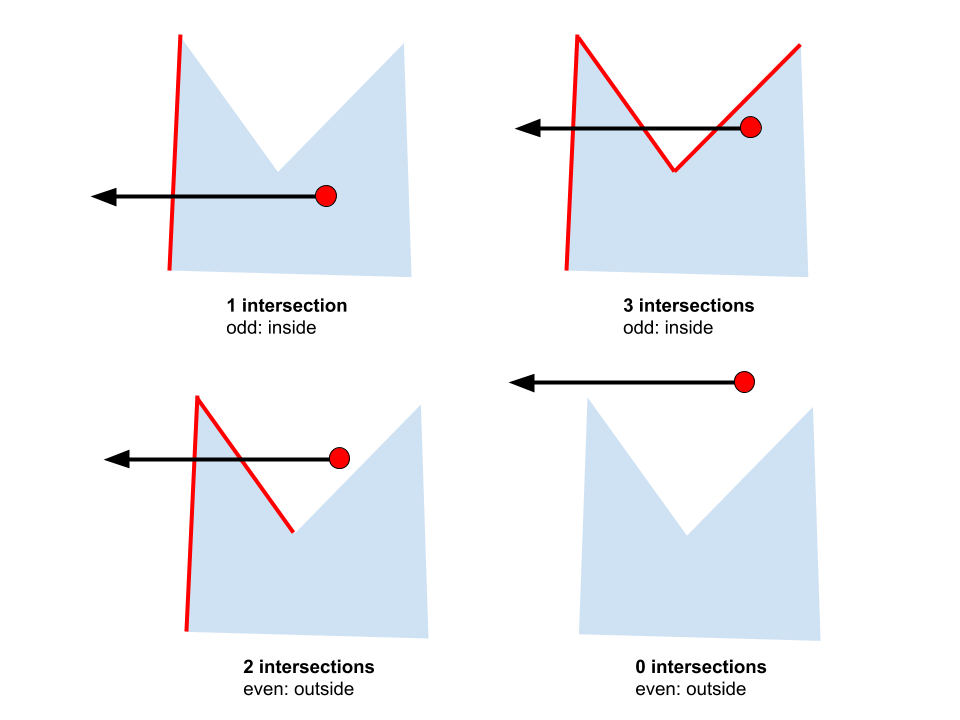
\includegraphics[width=0.7\textwidth]{intersections-diagram.png}
	\caption{A visualization of the algorithm}
	\label{fig:intersectionsDiagram}
\end{figure}

For this, we implemented a few mathematical functions for individual parts of
the algorithm, such as testing for intersection. We wrote unit-tests to test
each part of the algorithm, so we could be confident that the GPS component of
the app would correctly place users into the correct regions.

There is one edge case where this algorithm has difficulties. If the ray that
is drawn for testing intersections passes directly through a vertex, the
algorithm will count two intersections instead of just one. Even though this is
highly unlikely considering our use case, we decided that our algorithm should
be robust enough to handle this on a matter of principle. Unit-testing helped us
catch and deal with this edge case.

\subsection{Editour Frontend Testing}
\label{sec:editourFrontendTesting}

We suspect that Editour might have a life outside of this particular use case
for designing tours, depending on how we choose to further develop this
software. This is why Editour is perhaps more polished than your typical tool
purely for internal use.

For the duration of the project however, Editour only had to be used by us
three and Atticus. Therefore, the testing for the frontend of Editour was less
systematic than other parts of the software stack. This decision also helped us
focus our efforts on testing the reliability and user experience of ARuko. That
being said, we were able to add many feature and get the Editour experience to
a polished state through our own testing, using GitHub's tools to keep us
organized.

In order to test for bugs, all three of us periodically interacted with
successive builds of the frontend. When bugs were found, we would log these as
``Issues'' on the GitHub repo. These issues would get resolved in successive
pull requests.

Since we had to use Editour frequently to create test tours for ARuko, we were
able to identify features that would make our own work more efficient. This
worked as a kind of informal user testing. We kept track of feature requests
using the same system as bug reports.

Issues and feature requests alike got resolved in future pull requests. We
resolved over thirty issues and feature requests using this workflow. The
GitHub issues tab (which can be see in Figure~\ref{fig:issuesPageExample}) was
very useful for making sure we made use of our user testing and bug testing.

\begin{figure}[h]
	\centering
	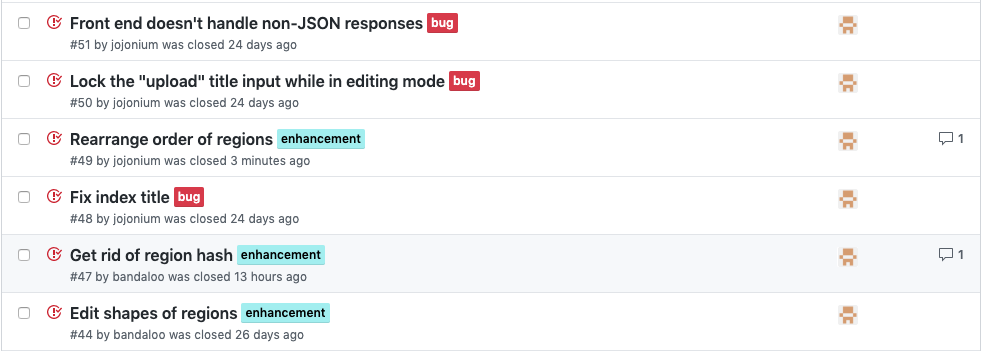
\includegraphics[width=\textwidth]{issues-page-example.png}
	\caption{The GitHub issues tab for Editour}
	\label{fig:issuesPageExample}
\end{figure}

\subsection{Testing Taking a Tour with ARuko}
\label{sec:testingARuko}

Because it was not feasible to travel to Kinkaku-ji every time we needed to
test the GPS functionality of the app, we used Editour to design an example
tour around the Ritsumeikan Biwako-Kusatsu campus where we worked. This allowed
us to catch various bugs before we created a finalized prototype for
field-testing at Kinkaku-ji. The tour represented in \ref{fig:ritsuTour} is
what we used for testing the app. The ``C-Shaped Region'' helped us test
concave regions. This uniquely shaped region also prompted us to think about
what UI behavior made the most sense if a user were to walk into a region, walk
out and then in again. We decided that it was awkward if the audio restarted
upon re-entering a region, since the audio would still be playing once a user
left the region. The region at the bottom surrounding our domitories was added
for our convenience, allowing us to test the app while we were away from the
lab.  As we began to implement more complex UI that changed based on GPS
position in various ways, directly taking the tour by walking around was an
invaluable way to test. Section~\ref{sec:adobeXdDesign} details how the UI grew
in complexity in the late stages of the project. Having a way to regularly run
field tests was integral to polishing the app in time before we revisited
Kinkaku-ji.  Because the Editour was flexible enough to easily swap out media
and add regions to the tour, the Editour proved itself to be as helpful for
testing as it was for crafting the final tour that could be taken at
Kinkaku-ji.

\begin{figure}[h]
	\centering
	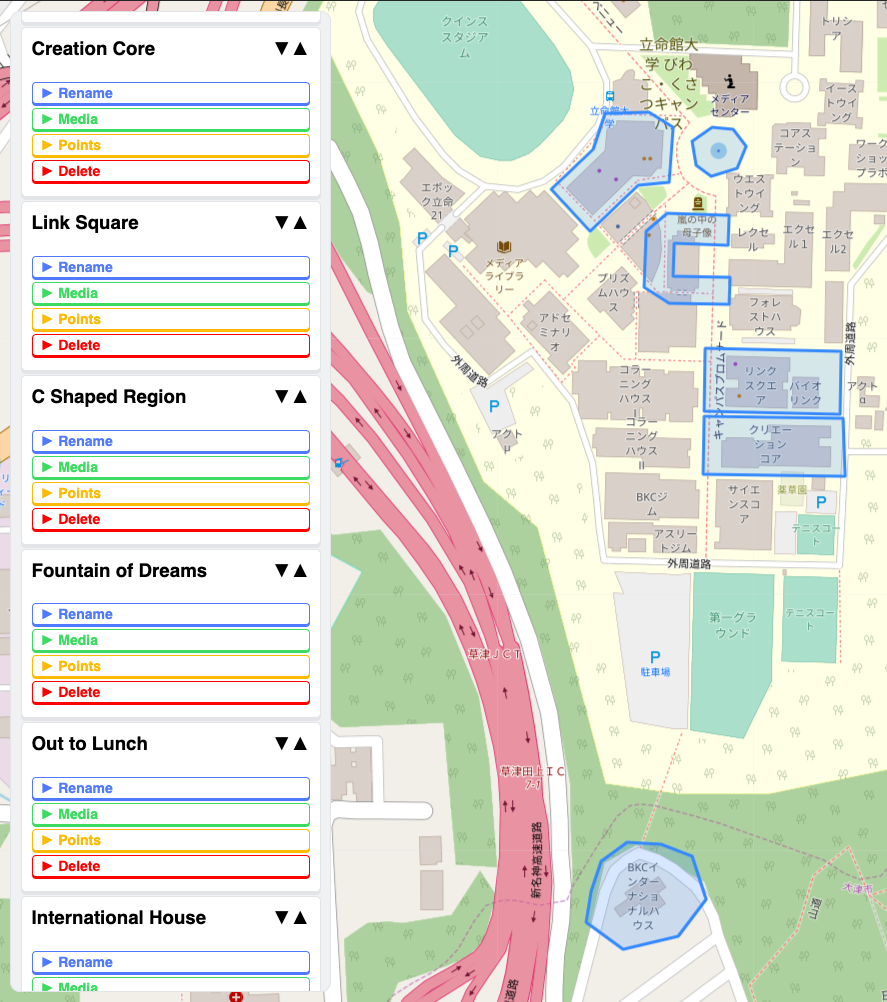
\includegraphics[width=.5\textwidth]{ritsu-tour.png}
	\caption{The Ritsumeikan example tour used for testing}
	\label{fig:ritsuTour}
\end{figure}

\subsubsection{First Round of Field Testing}
\label{sec:firstRoundOfFieldTesting}

Our first day of on-site testing with the app took place on September 6th.
Using Editour, we rebuilt the izi.TRAVEL audio tour that Atticus already
created. The first version of the rebuilt tour had regions that were relatively
small; some regions were only a few meters across. This version of the tour can
be seen in Figure~\ref{fig:kinkakujiTour}.

\begin{figure}[h]
	\centering
	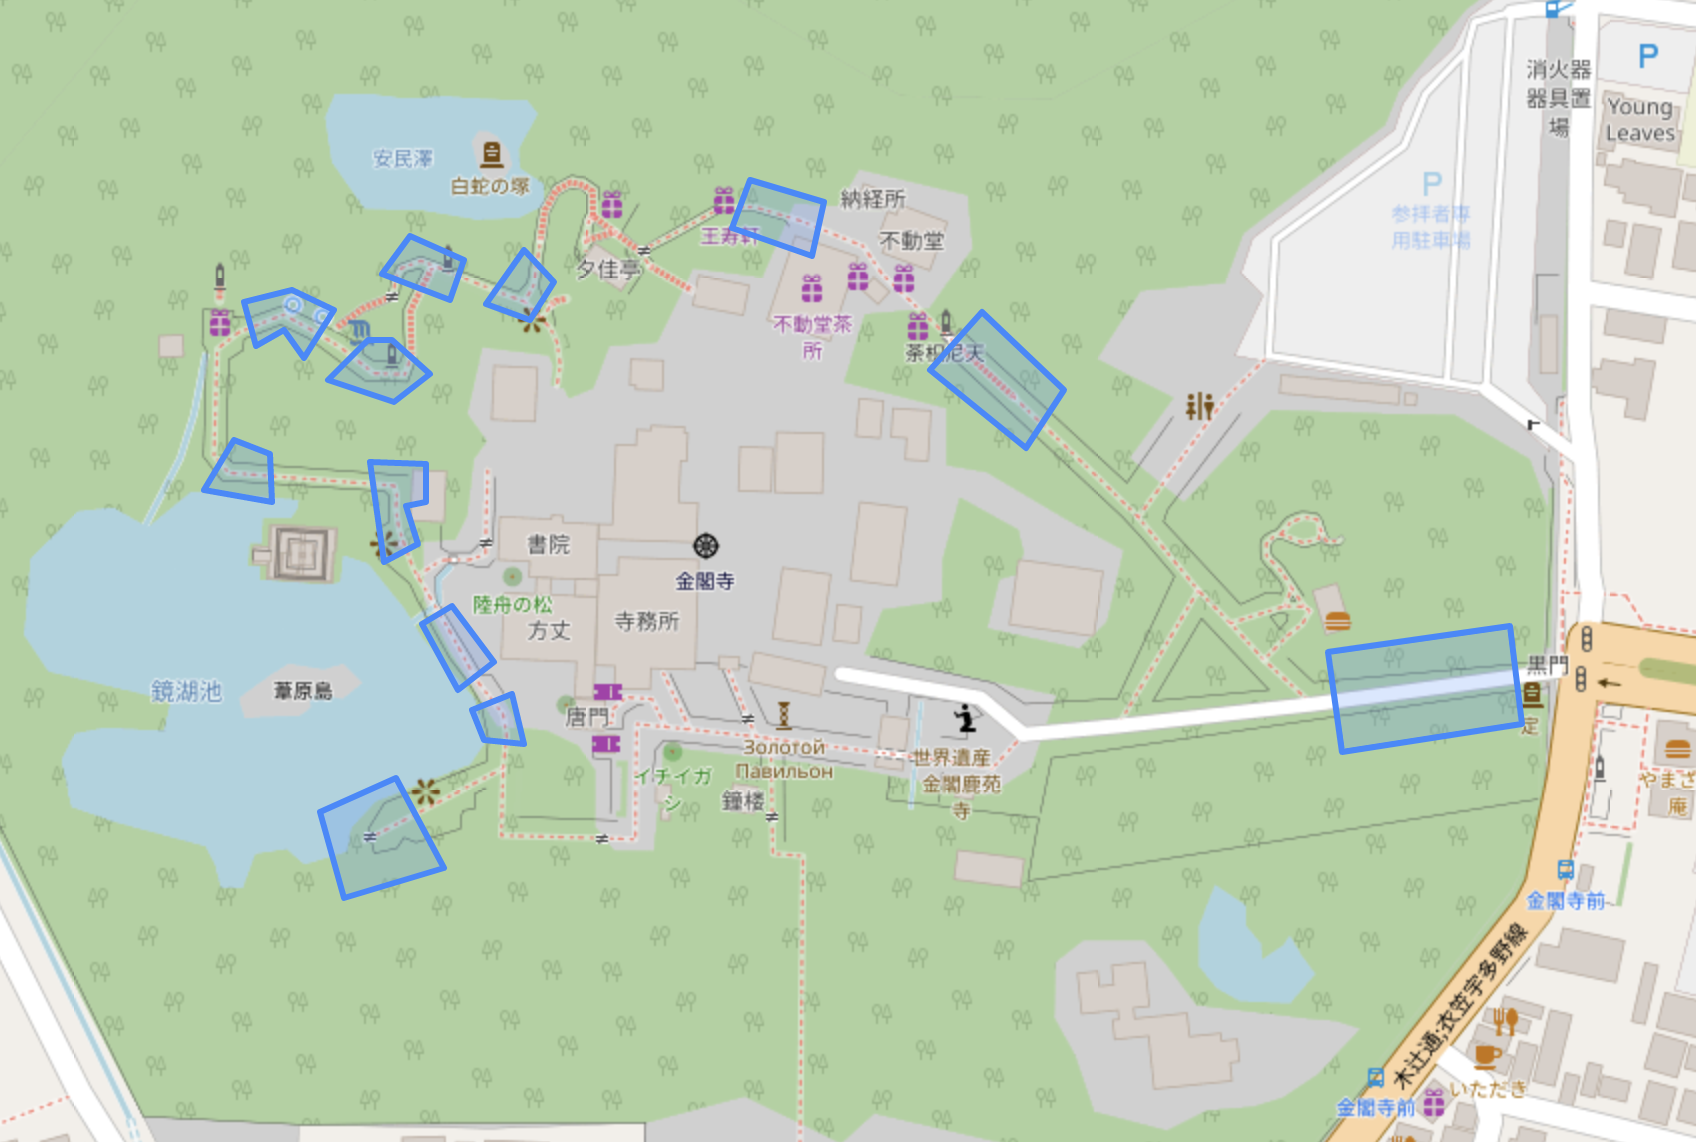
\includegraphics[width=\textwidth]{kinkakuji-tour.png}
	\caption[The original version of the Kinkaku-ji tour]{The original version
		of the Kinkaku-ji tour with small regions}
	\label{fig:kinkakujiTour}
\end{figure}

Due to concerns about GPS accuracy, we adapted the tour-file \texttt{kinkakuji}
to create a second, ``chunkier'' tour.  In the tour-file
\texttt{kinkakuji-chunkier}, we expanded all of the regions to accomodate for
potential GPS inaccuracies that could place the user outside the range of the
audio-trigger region.  Figure~\ref{fig:kinkakujiChunkierTour} depicts the tour
that we used for field testing at Kinkaku-ji.

\begin{figure}[h]
	\centering
	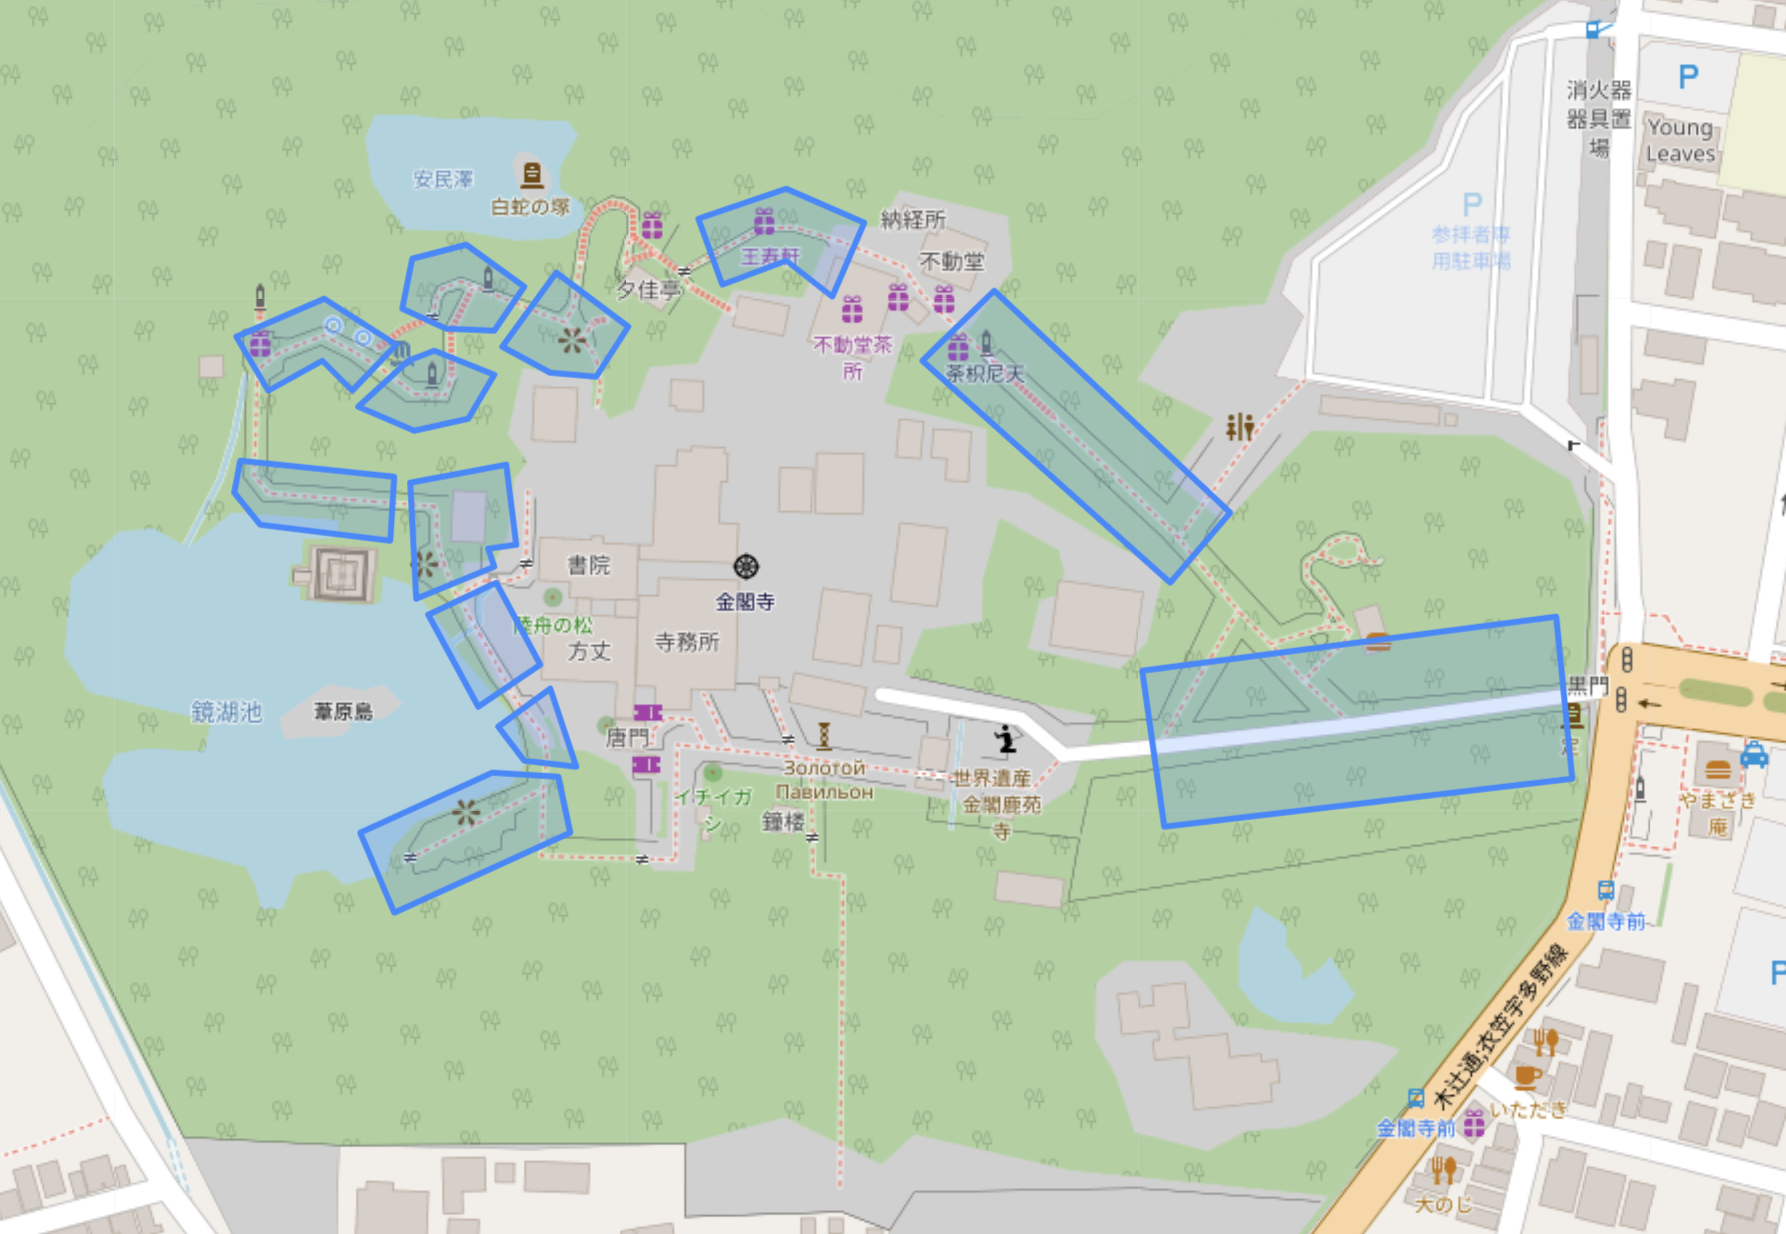
\includegraphics[width=\textwidth]{kinkakuji-chunkier-tour.png}
	\caption[The ``chunkier'' version of the Kinkaku-ji tour]{The ``chunkier''
		version of the Kinkaku-ji tour with larger regions}
	\label{fig:kinkakujiChunkierTour}
\end{figure}

We tested using two phones at the same time: an iPhone 8 and a Samsung Galaxy
S7. The iPhone 8 is newer, more powerful and therefore more suited for use with
AR. We primarily used this phone to test the AR features of the app. Even
though the Samsung Galaxy had difficulty with basic AR features such as
ground-plane detection, it was still capable of triggering the audio track
based on GPS position.

Our previous testing involved creating a ``mock tour'' on the Ritsumeikan
campus. While this let us know generally which features of the app were working,
it was very difficult to know how ahead of time how well our app would work at
Kinkaku-ji.

We were surprised by how intuitively each region triggered on the first try.
With a few exceptions, the audio started when the subject of the audio track
was in view. During our first walkthrough of Kinkaku-ji, we triggered every
region and audio track but one. The region that we missed on the first pass,
``Final Viewpoint'', requires the user to take a right at a fork in the road
instead of continuing along the main path. This is not necessarily a problem
with the design of the regions; instruction provided by the audio tour could
remedy this, directing the user toward the viewpoint that is off of the main
path.

Initially, we loaded the app onto the Samsung Galaxy S7 as a backup, since the
app is not fully functional on a phone that old. At the same time, it was
informative to take both phones through the tour. Initially, we made the design
decision to update the GPS location every 60 frames. On a phone running the app
at full speed, this should happen once every second. Because the Samsung Galaxy
S7 was having trouble running the app at full speed, the GPS updated far less
frequently. This was an oversight that would have been difficult to catch if we
had not tested on hardware below the recommended specifications.

Other bugs resulted from oversights that were difficult to catch with our
on-campus testing.  For example, we noticed that we forgot to back-up the audio
slider when entering a new region.  Because of this, when we entered a new
region when the audio slider was past the endpoint of the new audio track, the
audio would not play. For example, if the previous audio track were a minute
long, and if the second track were only thirty seconds long, the app would try
to play a thirty second audio track from the one minute mark. Since we were
running the app on phones, we could not easily see when errors were thrown.
Similarly, if the user were to enter a new region while thirty seconds into the
previous audio track, the new audio track would start at the thirty second
mark. During our on-campus testing, we were using songs rather than narration.
Since the songs were relatively long and not always obvious when they started
partway through, we did not catch this until we got out to Kinkaku-ji. Luckily,
this was trivial to fix.

% \begin{figure}[h]
%	\centering
%	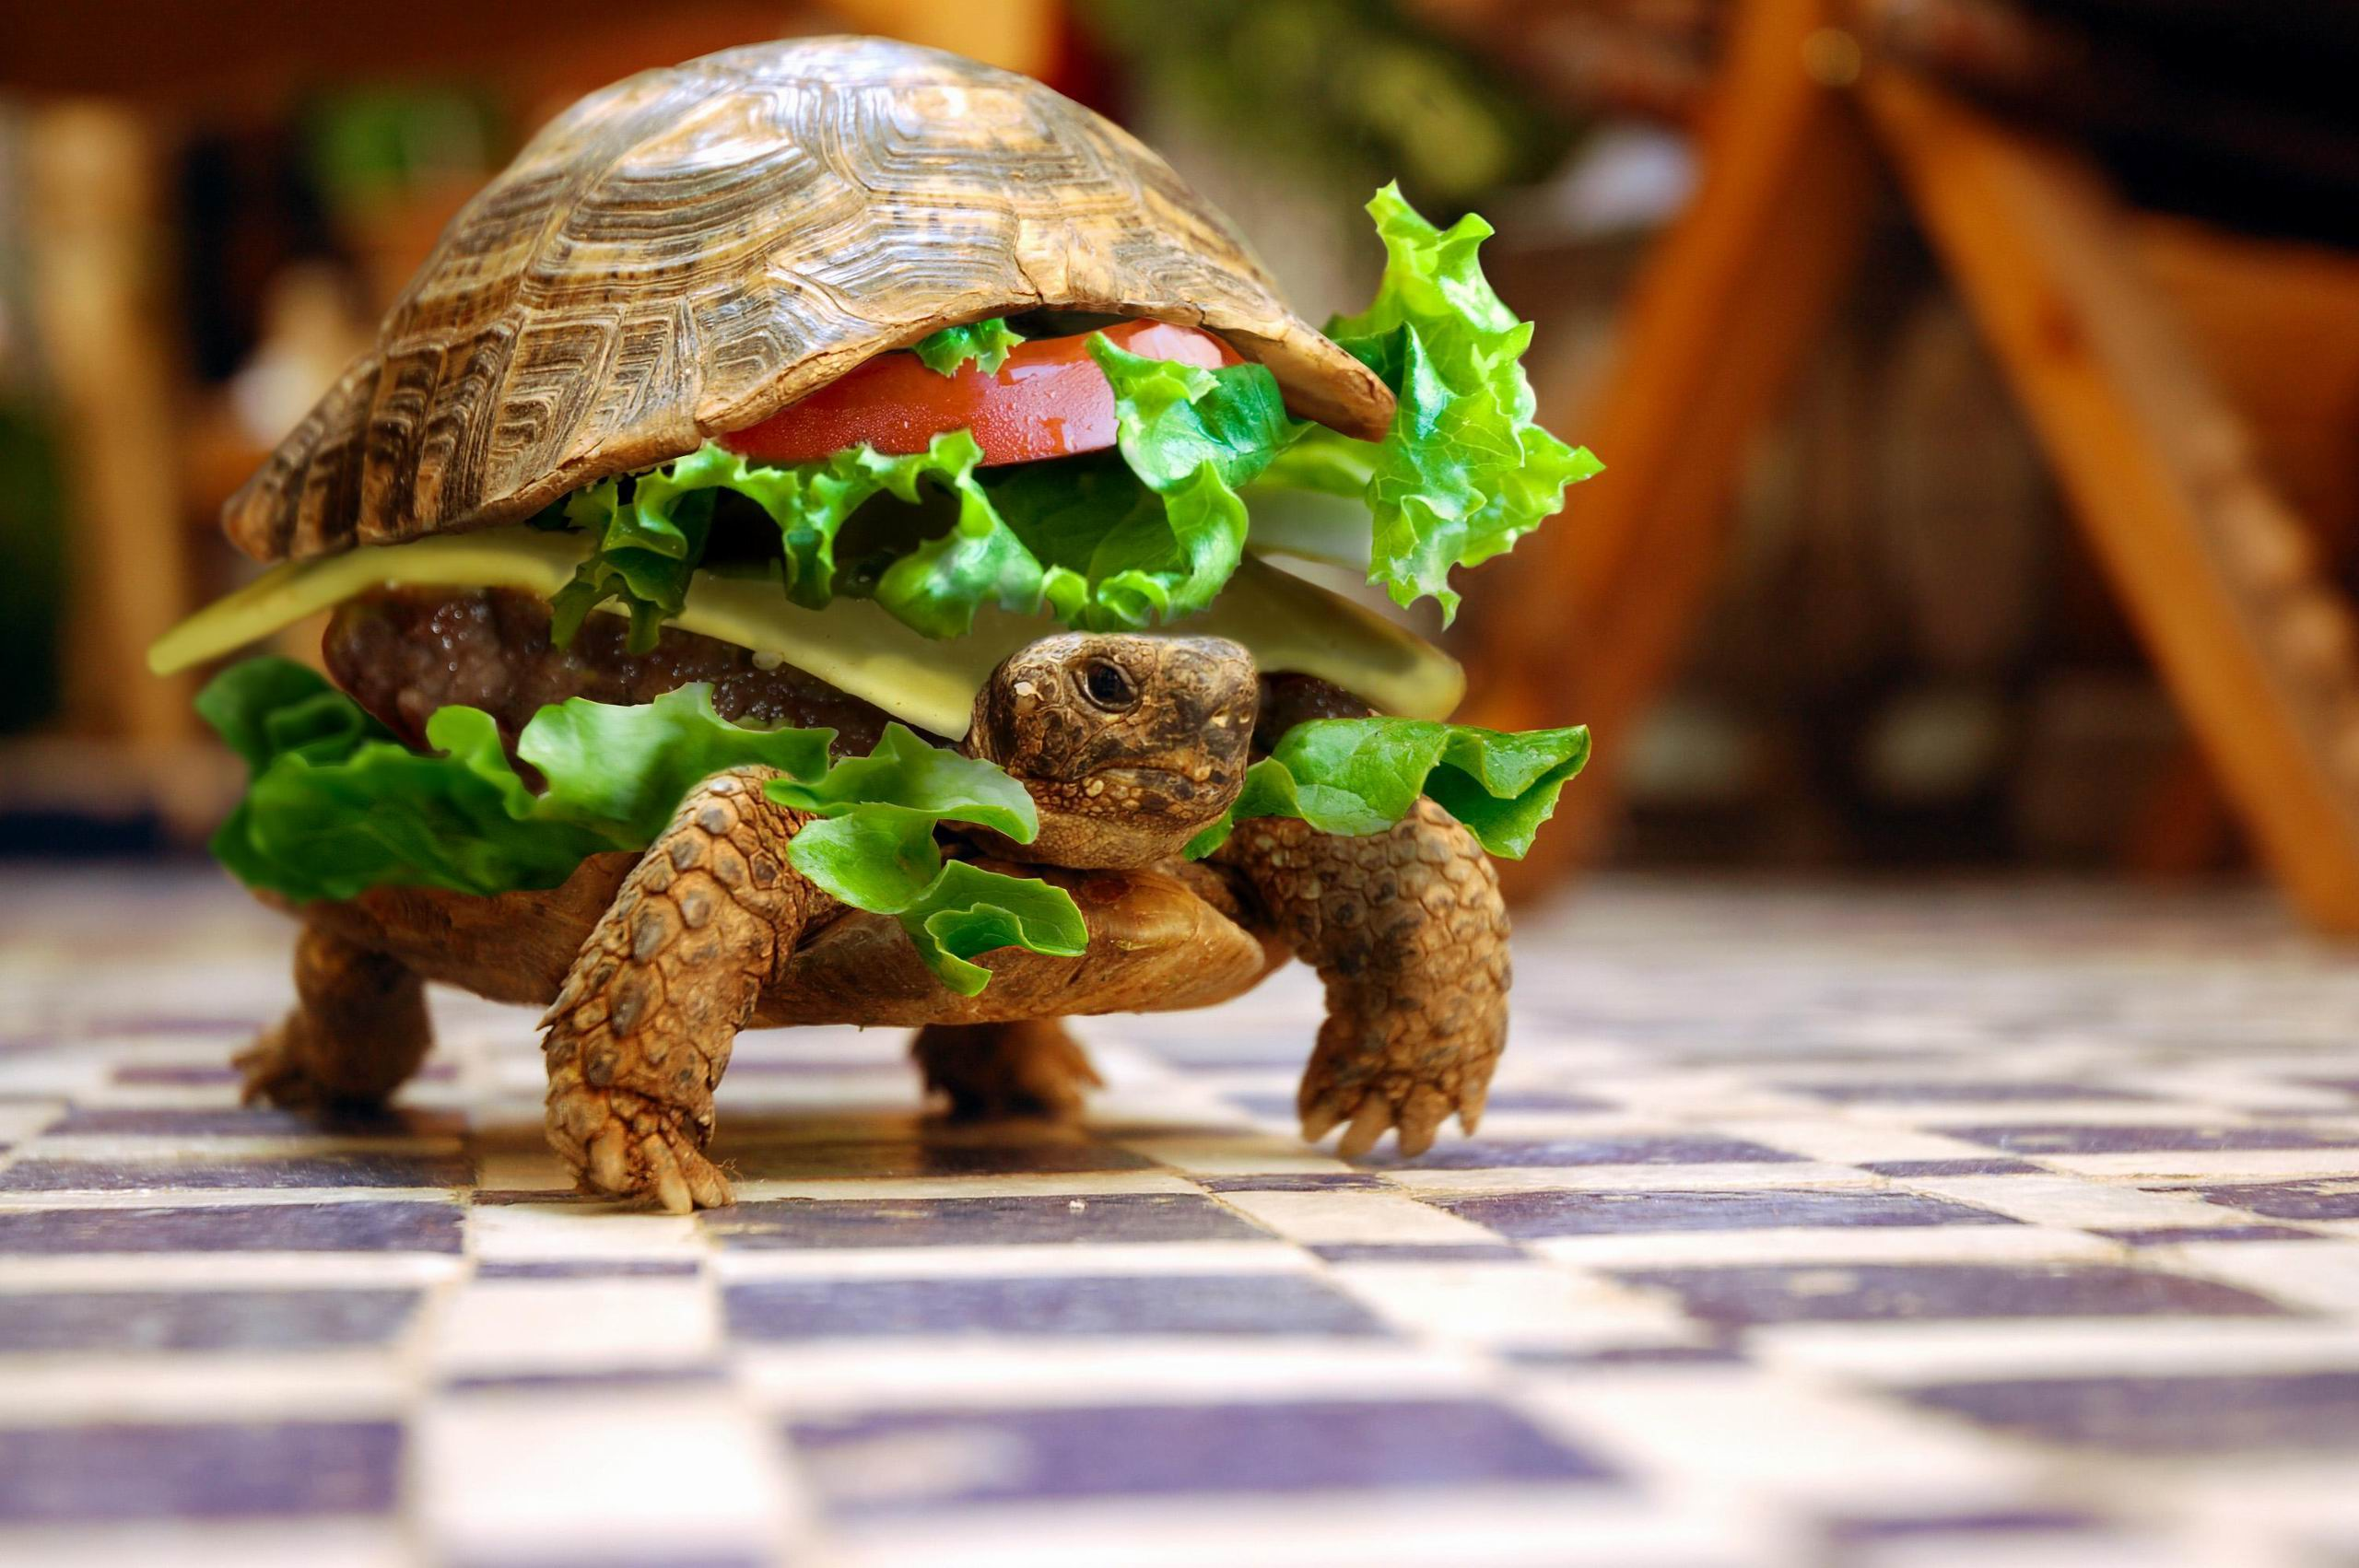
\includegraphics[width=\textwidth]{turtle-burger.jpg}
%	\caption[A rare but delicious turtle burger in the wild]{A rare but
%		delicious turtle burger in the wild~\autocite{harvey2002}.}
%	\label{fig:turtleBurger}
%\end{figure}

\newpage

\section{Pivots}
\label{sec:pivots}

Throughout the duration of the project, the goalposts shifted multiple times.
This section details some of the initial plans that fell through.

\newpage

\section{3D Spatialized Audio Tour}
\label{sec:3dSpatializedAudioTour}

\newpage

\section{Conclusion}
\label{sec:conclusion}

\nocite{harvey2002} % don't remove this

\newpage % references should be on their own page

\printbibliography
\addcontentsline{toc}{section}{References}

\newpage

\appendices
\section{Proof of the First Zonklar Equation}
Appendix one text goes here.

\section{}
Appendix two text goes here.

\end{document}


